\documentclass[10pt,twoside,final]{article}
\usepackage{wimnasu}
%\usepackage{layout}
%\usepackage{standalone}
%\usepackage{cmbright}
%\usepackage[T1]{fontenc}

%\newcommand{\pbf}[1]{\mbox{\mathversion{bold}$#1$}}

\DeclareMathOperator{\Hol}{Hol}
\DeclareMathOperator{\Arg}{Arg}
\DeclareMathOperator{\Ker}{Ker}
\DeclareMathOperator{\Res}{Res}
\DeclareMathOperator{\sinc}{sinc}



\begin{document}
	\let\oldenddocument\enddocument
	\let\document=\empty
	\let\enddocument=\empty
	\def\documentclass[#1]#2{\relax}
	\def\usepackage#1{\relax}

	%Show the page's layout 
	%\layout
	\selectlanguage{ukrainian} 
	
	
	%\graphicspath{./}{./ }
	%\tableofcontents
	\setcounter{page}{1}
	
	\subimportwork{Sytnyk/}{Sytnyk}
	\subimportwork{Mazko-Kupriyanchyk/}{Mazko-Kupriyanchyk}
	
	%\subimportwork{Mazko-Kupriyanchyk/}{Mazko-Kupriyanchyk}
	%\subimport{Mazko-Bogdanovich/}{Mazko-Bogdanovich}
	%\subimport{Fedunyk/}{Autor}
	%\subimport{Lila/}{Autor}
	%\subimport{Tkachenko/}{Tkachenko_2014}
	%\subimport{Timokha/}{Timokha_1}
	%\subimport{Timokha/}{Timokha_2}
	%\subimport{Trotsenko/}{Trotsenko_2014}
	%\subimport{Makarov-Romanyuk-Lazurchak/}{Makarov-Romanyuk-Lazurchak.tex}
	%\subimport{}{}
	%\subimport{}{}
	%\subimport{}{}
	%% !TeX encoding = windows-1251
\begin{document}
%%% ������ ��������������
\selectlanguage{ukrainian}

%\renewcommand{\ehkol}{�.�.~�����, �.�. ���������}
%\renewcommand{\ohkol}{������� ���������� � ������������� ������������� \dots}
%\aftergroup\clearpage
%\renewcommand{\thefootnote}{}
%\footnote {$^*$ ������ �������� �� ��������� ��������� ���
%�~0112U001015} \footnote{\hfill\copyright \ \ {\bf �.�.~�����, �.�. ���������, 2014}}
%
%\UDC{��� 517.935;519.718}
%%%% 517.9 - ����������������, ������������ � ������ �������������� ���������. �������� ��������. ������������ ����������. �������������� ������;
%%%% 517.925 - ������� � ������������� ������ ������������ ���������������� ���������;
%%%% 517.925.51 -  ������������ � ��������������� ��������� �������;
%%%% 517.93 - ����������� ���������������� ��������� � ������� ������������� ��������, ��������������� ����������, ����������� � ������������ �������;
%%%% 517.935 - ��������� ������ ��������������� ����������;
%%%% 517.983.27 - �������� ��������� � ����������������� �������������;
%%%% 519.71 - ������ ����������� ������ (�������������� �������);
%%%% 519.711 - ����� ������� ������ ����������� ������;
%%%% 519.715 - ������� ������� � ������ ����������� ������;
%%%% 519.718 - ������������, ���������� � ��������;
%
%\vspace*{-3mm}
%\Title{������� ���������� � ������������� ������������� �� ��������� ��������� ��'�����\,$^*$}
%%\label{Mazko-Kupriyanchyk:FirstPage}}
%
%\Author{\large �.�.~�����, �.�. ���������}
%\Address{�������� ���������� ��� ������, ���;  mazko@imath.kiev.ua}
%\medskip
%
%\AbsEng{The work is devoted to working out of new methods for analysis of robust stability,
%stabilization and optimization of the equilibrium states of nonlinear dynamic  output feedback control systems. It is shown that stabilization and optimization problems with dynamic output feedback are reduced to analogical problems with static output feedback. Sufficient stability conditions of the zero solution are formulated with the joint quadratic Lyapunov function for a family of nonlinear systems with uncertain coefficient matrices and a measured output feedback. The solution of general problem of robust stabilization and evaluation of the quadratic performance criterion for the family of nonlinear systems are proposed. Applying the results reduces to solving the finite systems of linear matrix inequalities.}
%\AbsRus{������ ��������� ���������� ����� ������� ������� ��������� ������������, ������������ � ����������� ��������� ���������� ���������� ������ ���������� � ������������ �������� ������ �� ����������� ������. ��������, ��� ������ ������������ � ����������� � ������������ �������� ������ �������� � ����������� ������� �� ����������� �������� ������. ��� ��������� ���������� ������ � ��������������� ��������� ������������� � �������� ����� �� ����������� ������ ������������� ����������� ������� ������������ �������� ��������� � ����� ������������ �������� ��������. ������������ ������� ����� ������ ��������� ������������ � ������ ������������� �������� �������� ��������� ���������� ������. ���������� ���������� ����������� �������� � ������� �������� ������ �������� ��������� ����������.}
%
\udc{517.935;519.718}
\title[������� ���������� � ������������� ������������� �� ��������� ��������� ��'�����]{������� ���������� � ������������� ������������� �� ��������� ��������� ��'�����%}
\thanks{������ �������� �� ��������� ��������� ��� �~0112U001015}}
%\label{Mazko-Kupriyanchyk:FirstPage}}

\author{�.�.~�����, �.�. ���������}
\address{�������� ���������� ��� ������, ���;  mazko@imath.kiev.ua}

\abstractru{������ ��������� ���������� ����� ������� ������� ��������� ������������, ������������ � ����������� ��������� ���������� ���������� ������ ���������� � ������������ �������� ������ �� ����������� ������. ��������, ��� ������ ������������ � ����������� � ������������ �������� ������ �������� � ����������� ������� �� ����������� �������� ������. ��� ��������� ���������� ������ � ��������������� ��������� ������������� � �������� ����� �� ����������� ������ ������������� ����������� ������� ������������ �������� ��������� � ����� ������������ �������� ��������. ������������ ������� ����� ������ ��������� ������������ � ������ ������������� �������� �������� ��������� ���������� ������. ���������� ���������� ����������� �������� � ������� �������� ������ �������� ��������� ����������.}

\abstracten{The work is devoted to working out of new methods for analysis of robust stability,
	stabilization and optimization of the equilibrium states of nonlinear dynamic  output feedback control systems. It is shown that stabilization and optimization problems with dynamic output feedback are reduced to analogical problems with static output feedback. Sufficient stability conditions of the zero solution are formulated with the joint quadratic Lyapunov function for a family of nonlinear systems with uncertain coefficient matrices and a measured output feedback. The solution of general problem of robust stabilization and evaluation of the quadratic performance criterion for the family of nonlinear systems are proposed. Applying the results reduces to solving the finite systems of linear matrix inequalities.}
 
%\footnote{\hfill\copyright \ \ {\bf �.�.~�����, �.�. ���������, 2014}}
\maketitle

%\setcounter{page}{100}
\section{�����}
��� ������������ ������������, �������� �� ����� ��������� ��'���� ��������� �������� ������� ������������ ������ �� ����� ������, �� �������� �� ���. �������� ������� ��������� � ����� ������� ��������� ���������� ��������� ����� �� �������� ������ ���������. �����, � �������� ��'����� �������� �������� ������������� ����� ���� �� ��������� ���������� ��� �� ����. ���� �� �� ����������� ��� ������� ���������  ������������ �������, �� ������� ��������� ������ ��'������ � �������� ������ ���� �� ������������� ������� ��������� ����� �, �������, �������.
������������� � ����������� �� ���������� ������������ ������� ��������� ������ ���������� �����������, ���������, �������� �� ������������� ��'��� ������� ���� (���., ���������, \cite{Polyak-Scherbakov,Zhou-Doyle-Glover,Kuncevich,Polyak-Scherbakov-1,Aliev-Larin}). ��� ����� ������������� ������ � ����������������� ��������� ����� ��������������� ������� �������� �� ��������� \cite{Mazko-2008, Mazko-2011}.

�������� ���� $x\equiv 0$ �������� �������������� ������� ��������� � ������������� ��������������
\begin{equation}\label{f1-1}
\dot{x}=f(x,p,t)+B(x,p,t)\,u,\quad f(0,p,t)\equiv 0,\quad u=K x,\quad x\in {\mathbb R}^n,
\end{equation}
�� $f(\cdot)$ � $B(\cdot)$ --- �������� �������� �� �������� �������, ���������� \emph{�������� ������} ������� ������� ������ ��������� ${\mathcal P}\subseteq {\mathbb R}^\nu$ �� ����������� ������� ��������� ���������� ��'���� ${\mathcal K}\subset {\mathbb R}^{m\times n}$, ���� �� ������������ ������ �� ��������� ��� ��� ���������� $p\in{\mathcal P}$ � $K\in {\mathcal K}$. ��������-�������� ������� ��������� ���� (\ref{f1-1}) ���� ��������� ��������. ���� $f(x,p,t)=A(x,p,t)\,x$, �� $A(\cdot)$ --- �������� �������, �� ��� ���������� ����� �������� ������� �� ���������� ������� (\ref{f1-1}) ������ ������ ��������������� ������ ������������ ������� �������� $v(x,t)=x^TX(t)x$ � ����������� ������� ���������� �������� $X(t)$.

 � ��������� ������� � ������� ������� ��������� ���������� (���) �������� �������� ����� ������� ������� ��������� ������ � ������������� ��������� ����������� � ���������� ��'���� �� ����������� ������. � ������� ����� � ������ ������ ������ �������� ������� � ���������� ������ ��������� � ��������� ��'����� ����� ������������� � ������� \cite{Polyak-Scherbakov-1,Aliev-Larin}.

���� ������ ���������� �������� ����� ������ ������ �������� �������, ���������� �� ���������� ������ �������� ����� ��������� ������������� ������ ��������� � ��������� ��������� ��'����� �� ����������� ������, �� ������ ���������� �� ������� ������, ��� � ���������. ��������, �� ������ ���������� �� ���������� � ��������� ��������� ��'����� (���) ��������� �� ���������� ����� � ��������� ��������� ��'����� (���). �������������� � ���������� ���������� ���� \cite{Balandin-Kogan,Maz-Shram-2011,Mazko-2011-IM,Maz-Bog-2012}, ������������ �������� ����� ������� ��������� ����� ��'� ������ ��������� � ������������� ��������� ����������� � ��� �� ����������� ������. ����� ��������� ������ ������� �������� � ������ ������ ������������� ����������� �����. � ��������� ������������ ��� ������
���������� ���� ��'� ������. ��������� ������������ ��������� ���������� ��������� �� ����������� ����'���� ������ ��������������� ��� ����������� ���. ��� ����'������ ��� � ������� ��������� ���� ���� ����������� ������ ��������� ��������� � ������ {\sc Matlab} \cite{Gu-Petkov-Konstantinov}.

������ ��������������� ��� ����������: $I_n$ --- �������� ������� ������� $n$;
$0_{n\times m}$ --- ������� ������� ������ $n\times m$;
 $X=X^T>0$ $(\ge 0)$ --- ������� (����'����) ��������� ���������� ������� $X$;
$i(X)=\{i_+,i_-,i_0\}$ --- ������� ������� ������� $X$, ��� ��������� ������� �� ��������, ��'����� � �������� ������� �������, ���������� ��������;
$\lambda_{\max}(X)$ ($\lambda_{\min}(X)$) --- ����������� (���������) ������ �������� ������� ������� $X$;
 $\rho(A)$ --- ������������ ����� ������� $A$;
$\|x\|$ --- �������� ����� ������� $x$;
${\rm Co}\{A_1,\dots,A_\nu\}$ --- ������� ������������ (������) � ��������� $A_1,\dots,A_\nu$ � ������� ������� �������
$${\rm Co}\{A_1,\dots,A_\nu\}=\Big\{A=\sum_{i=1}^\nu \alpha_i A_i:\>\>\alpha_i \ge 0,\>i=\overline{1,\nu},\>\sum_{i=1}^\nu \alpha_i=1\Big\}.$$

\section{���������� ������� ������ ���������\\ � ��������� �����������}

 ���������� ������� ���������
\begin{equation}\label{s1-1}
\dot{x}=Ax+Bu,\quad y=Cx+Du,
\end{equation}
�� $x\in {\mathbb R}^{n}$, $u\in {\mathbb R}^{m}$ � $y\in {\mathbb R}^{l}$ --- ������� �������� �����, ��������� �� ������������� ��'����, $A$, $B$, $C$ � $D$ --- ������� ��������� ������ $n\times n$, $n\times m$, $l\times n$ � $l\times m$, �������, $\rm rank\,B=m$ � $\rm rank\,C=l$.
�������� ��������� ��������� � ������ ���
\begin{equation}\label{s1-2}
\begin{cases}
\dot{z}=Zz+Vy, \\
u=Uz+Ky,
\end{cases}
\end{equation}
�� $z\in {\mathbb R}^{r}$ --- ������ ����� ����������, $Z$, $V$, $U$ � $K$ --- ������ ������� ��������� ������ $r\times r$, $r\times l$, $m\times r$ � $m\times l$. � �������� ������� $r=0$ ���� ��������� ��������� $u=Ky$. ��� $r\neq0$ ������������ (\ref{s1-1}) � (\ref{s1-2}) ����� �������� � ����������� ������:
\begin{equation}\label{s1-3}
\dot{\widehat{x}}=\widehat{A}\widehat{x}+\widehat{B}\widehat{u},\quad \widehat{y}=\widehat{C}\widehat{x}+\widehat{D}\widehat{u},\quad  \widehat{u}=\widehat{K}\widehat{y},
\end{equation}
��
$$
\widehat{x}=\left[\!\begin{array}{c}
              x \\
              z
              \end{array}
               \!\right],\quad
\widehat{y}=\left[\!\begin{array}{c}
              z \\
              y
              \end{array}
               \!\right],\quad
\widehat{u}=\left[\!\begin{array}{c}
              \dot{z} \\
              u
              \end{array}
               \!\right],
               \quad
\widehat{K}=\left[\!\begin{array}{cc}
                            Z & V \\
                            U & K
                            \end{array}
                            \!\right],
               $$$$
\widehat{A}=\left[\!\begin{array}{cc}
              A & 0_{n\times r} \\
              0_{r\times n} & 0_{r\times r}
              \end{array}
               \!\right],\quad
\widehat{B}=\left[\!\begin{array}{cc}
              0_{n\times r} & B \\
              I_r & 0_{r\times m}
              \end{array}
               \!\right],
$$
$$
\widehat{C}=\left[\!\begin{array}{cc}
              0_{r\times n} & I_r \\
              C & 0_{l\times r}
              \end{array}
               \!\right],\quad
\widehat{D}=\left[\!\begin{array}{cc}
              0_{r\times r} & 0_{r\times m} \\
              0_{l\times r} & D
              \end{array}
               \!\right],
$$
�������, ${\rm rank}\,\widehat{B}=r+m$ � ${\rm rank}\,\widehat{C}=r+l$.
� ������ ����, ���� �������� $u=Uz+Ky$, ��, ���������� ��������� ������� ������� � (\ref{s1-3}), �������� �� ������������ (\ref{s1-1}) � (\ref{s1-2}).
\begin{lemma}\label{lem:1}
������� ��������� {\rm (\ref{s1-1})} � ��������� ����������� {\rm (\ref{s1-2})} ������� $r\ne 0$ ����������� ������ ��������� � ��� {\rm (\ref{s1-3})}.
\end{lemma}

����� �����, ������ ��������� �, �������, ���������� ������� (\ref{s1-1}) � ��� (\ref{s1-2}), ��������� �� ���������� ����� ��������� ��� ������� (\ref{s1-3}) � ���.

������� �� ������� ������� ${\mathcal K}_{\widehat{D}}=\{\widehat{K}:\det(I_{r+m}-\widehat{K}\widehat{D})\ne 0\}$ ��������� ��������
$$
\mathcal{\widehat{D}}:\,{\mathbb R}^{(r+m)\times (r+l)}\rightarrow{\mathbb R}^{(r+m)\times (r+l)},\quad \mathcal{\widehat{D}}(\widehat{K})= (I_{r+m}-\widehat{K}\widehat{D})^{-1}\widehat{K},$$
��� � �������� ������
$$\mathcal{\widehat{D}}(\widehat{K})=
 \left[\begin{array}{c|c}
                        Z+VD(I_m-KD)^{-1}U & V(I_l-DK)^{-1} \\
                        \hline
                        (I_m-KD)^{-1}U & \mathcal{D}(K)
                        \end{array}
                        \right],$$
 �� $\mathcal{D}(K)=(I_m-KD)^{-1}K$,\,\, $K\in {\mathcal K}_D=\{K:\det(I_m-KD)\ne 0\}$.

��� ����� ������� ���������� ��'���� $\widehat{K}\in {\mathcal K}_{\widehat{D}}$ �������� ������� (\ref{s1-3}) �� ������
\begin{equation}\label{s1-4}
\widehat{\dot{x}}=\widehat{M}\,\widehat{x},\quad \widehat{M}=\widehat{A}+\widehat{B}\mathcal{\widehat{D}}(\widehat{K})\widehat{C},
\end{equation}
��
$$\widehat{M}\!=\!
 \left[\begin{array}{c|c}
                        M & B(I_m-KD)^{-1}U \\
                        \hline
                        V(I_l-DK)^{-1}C & Z+VD(I_m-KD)^{-1}U
                        \end{array}
                        \right],\> M\!=\!A+B\mathcal{D}(K)C.$$

�������� $\mathcal{\widehat{D}}$ �� ��� ����������:\\[2mm]
\noindent $\bullet$ ���� $\widehat{K}\in{\mathcal K}_{\widehat{D}}$, �� $\mathcal{\widehat{D}}(\widehat{K})\equiv\widehat{K}(I_{r+l}-\widehat{D}\widehat{K})^{-1}
\equiv
\widehat{K}[I_{r+l}+\widehat{D}\mathcal{\widehat{D}}(\widehat{K})]$,
$
I_{r+l}+\widehat{D}\mathcal{\widehat{D}}(\widehat{K})\equiv (I_{r+l}-\widehat{D}\widehat{K})^{-1};
$

\noindent $\bullet$ ���� $K_1\in{\mathcal K}_{\widehat{D}}$, $K_2\in{\mathcal K}_{\widehat{D}_1}$, �� $K_3=(I_{r+m}-K_1\widehat{D})^{-1}K_2\in{\mathcal K}_{\widehat{D}}$, $K_1+K_2\in{\mathcal K}_{\widehat{D}}$ �
\begin{equation}\label{s1-6}
\begin{array}{c}
  \widehat{{\mathcal D}}(K_1+K_2)= \widehat{{\mathcal D}}(K_1)+\widehat{{\mathcal D}}(K_3)\,(I_l-\widehat{D}K_1)^{-1}, \\[2mm]
  \widehat{{\mathcal D}}(K_3)=(I_m-K_1\widehat{D})^{-1}\widehat{{\mathcal D}}_1(K_2),
\end{array}
\end{equation}
�� $\widehat{D}_1=(I_l-\widehat{D}K_1)^{-1}\widehat{D}$,\,\, $\widehat{{\mathcal D}}_1(K_2)=(I_m-K_2\widehat{D}_1)^{-1}K_2$;

\noindent $\bullet$ ���� $\widehat{K}\in{\mathcal K}_{\widehat{D}}$, �� $\widehat{K}_*=-\mathcal{\widehat{D}}(\widehat{K})\in {\mathcal K}_{\widehat{D}}$ �
\begin{equation}\label{s1-7}
 \mathcal{\widehat{D}}(\widehat{K}_*)= - \widehat{K}.
\end{equation}

����� � (\ref{s1-7}), ��� ���������� ������� ������������ �, �������, ������� ������� (\ref{s1-4}) ��������� ����������� �� ���������� ������
\begin{equation}\label{s1-4-1}
\widehat{\dot{x}}=\widehat{M}\,\widehat{x},\quad \widehat{M}=\widehat{A}-\widehat{B}\widehat{K}\widehat{C},
\end{equation}
��� ���� $\widehat{K}\in{\mathcal K}_{\widehat{D}}$.
��� ������� ������� ����� $\widehat{B}$ � $\widehat{C}$ ��������� ������������ ���������� � �������������� �������:
$$\widehat{B}^{\bot}=\left[\!\begin{array} {c}
                        B^{\bot}\\
                        0_{r\times(n-m)}
                        \end{array}
                        \!\right],\quad
\widehat{B}^+=(\widehat{B}^T\widehat{B})^{-1}\widehat{B}^T=\left[\!\begin{array}{cc}
                                                 0_{r\times n} & I_r \\
                                                B^+ & 0_{m\times r}
                                                \end{array}
                                                 \!\right],$$
$$\widehat{C}^{\bot}=\left[C^{\bot}, 0_{(n-l)\times r}\right],\quad
\widehat{C}^+=\widehat{C}^T (\widehat{C} \widehat{C}^T)^{-1}=\left[\!\begin{array}{cc}
                                                0_{n\times r} & C^+ \\
                                                 I_r & 0_{r\times l}
                                                  \end{array}
                                               \!\right],$$
�� $\det\big[\widehat{B},\widehat{B}^{\bot}\big]\ne 0$, $\widehat{B}^T\widehat{B}^{\bot}=0$,
$\det \big[\widehat{C}^T,\widehat{C}^{\bot T}\big] \neq 0$, $\widehat{C}\widehat{C}^{\bot T}=0$.

�������� ���������� �� �������� �������� ������� ������� (\ref{s1-4-1}) � �������� ������������� ������� ����� ${\rm Re}\,\lambda =\alpha$, $\lambda\in {\mathbb C}^1$.

\begin{lemma}\label{lem:2} ���� ������� $\widehat{K}$, ��� ��� ������ ������� (\ref{s1-4-1}) ���������� �� $p$ � $q$ ����� � ��������� ������������ ${\rm Re}\,\lambda <\alpha$ � ${\rm Re}\,\lambda >\alpha$, ��� � ���� ���, ���� ������ �������
$\widehat{X}=\widehat{X}^T$
������� �����������
\begin{equation}\label{s1-8}
S=B^{\bot T}LB^{\bot}<0,\quad i(\widehat{X})=\{p,q,0\},\quad
i(\widehat{H})=\{r+l,r+m,0\},
\end{equation}
��
$$L=AX+XA^T-2\alpha X,\quad \widehat{X}=\left[\!\begin{array}{cc}
                        X & X_1^T \\
                        X_1 & X_2
                        \end{array}
                        \!\right],\>\>\widehat{H}=\left[\begin{array}{cc}
      \widehat{H}_0 & \widehat{H}_1^T \\
     \widehat{H}_1 & \widehat{H}_2
       \end{array}\right],$$
$$ \widehat{H}_0=
         \left[ \begin{array}{c|c}
                        -2\alpha X_2-X_1A_\alpha^T RA_\alpha X_1^T & X_1A_\alpha^T(I_n-RL)B^{+T} \\
                        \hline
                        B^+(I_n-LR)A_\alpha X_1^T & H_0
                        \end{array}
                         \right],$$
$$\widehat{H}_1=
       \left[ \begin{array}{c|c}
                        X_2-X_1RA_\alpha X_1^T & X_1(I_n-RL)B^{+T} \\
                        \hline
                        C(I_n-XRA_\alpha)X_1^T & H_1
                        \end{array}
                         \right],$$
$$\widehat{H}_2=
       \left[ \begin{array}{c|c}
                        -X_1RX_1^T & -X_1RXC^T \\
                        \hline
                        -CXRX_1^T & H_2
                        \end{array}
                         \right],$$
$$H_0=B^+(L-LRL)B^{+T},\>\>\> H_1=CX(I_n-RL)B^{+T},\>\>\> H_2=-CXRXC^T,$$
$$R=B^{\bot}S^{-1}B^{\bot T},\quad  A_\alpha=A-2\alpha I_n.$$

�� ���� {\rm (\ref{s1-8})} ������� $\widehat{K}$ ���� ���� �������� �� ����'���� ������ �� ������������ ��������� ����������
\begin{equation}\label{s1-9}
\widehat{H}_0-\widehat{K}\widehat{H}_1-\widehat{H}_1^T\widehat{K}^T+\widehat{K}\widehat{H}_2\widehat{K}^T<0,
\end{equation}
\begin{equation}\label{s1-10}
\widehat{A}\widehat{X}+\widehat{X}\widehat{A}^T-2\alpha \widehat{X}<\widehat{B}\widehat{K}\widehat{C}\widehat{X}+\widehat{X}\widehat{C}^T\widehat{K}^T\widehat{B}^T.
\end{equation}
�������, ���� � ������������� {\rm (\ref{s1-8})} � {\rm (\ref{s1-9})} $\widehat{X}=\widehat{X}^T>0$, $\alpha\le 0$, �� ������� (\ref{s1-4-1}) ������������ �����.
\end{lemma}

���� ���� ������� �� ���� ��������� ����������� � ����������� ����������, ������������� � \cite{Maz-Bog-2012} ��� ��������� ����������. ���������, �� ������ ������� $\widehat{K}$ ��������� (\ref{s1-10}) ����������, ����
$$
\widehat{K}=\widehat{B}^T\widehat{X}^{-1}\widehat{C}^+,\>
\widehat{A}\widehat{X}+\widehat{X}\widehat{A}^T-2\alpha \widehat{X}< 2\,\widehat{B}\widehat{B}^T,\> (\widehat{C}^+\widehat{C}-I_{r+n})\widehat{X}^{-1}\widehat{B}=0,
$$
� ��� ��������� ����������� ������� $\widehat{K}$ �������� (\ref{s1-9}) ���������
\begin{equation}\label{s1-12}
\widehat{K}= \gamma\, \widehat{B}^T\widehat{X}^{-1}\widehat{C}^+, \quad \gamma > \lambda_{\max}(\widehat{H}_0)/2,\quad \widehat{C}^{\bot}\widehat{X}^{-1}\widehat{B}=0,
\end{equation}
�������, ������� ������ � ��������� ������������� �����������.

���������� (\ref{s1-7}) � (\ref{s1-12}), ��� $\alpha\le 0$ ���� �������� �����, �� ���������� ������������ ������� ������� (\ref{s1-4}) � ������������ �������, �� ������, ��� $|\alpha|$:
$$
  \widehat{X}=\widehat{X}^T>0, \quad  \widehat{B}^{\bot T}(\widehat{A}\widehat{X}+\widehat{X}\widehat{A}^T-2\alpha \widehat{X})\,\widehat{B}^{\bot}<0,\quad \widehat{C}^{\bot}\widehat{X}^{-1}\widehat{B}=0,
$$
\begin{equation}\label{s1-13}
  \widehat{K}=-\mathcal{\widehat{D}}(\widehat{K}_*),\quad  \widehat{K}_*=\gamma\, \widehat{B}^T\widehat{X}^{-1}\widehat{C}^+\in \mathcal{K}_{\widehat{D}},\quad \gamma >  \lambda_{\max}(\widehat{H}_0)/2.
\end{equation}

��� ������� (\ref{s1-3}) � �������� $D=0$ ����������� �������� ����������. ���� ������� ���������� ���������� ��'���� $\widehat{K}$ ����, �� �������� ������� (\ref{s1-4}) ������������ �����, ��� � ���� ���, ���� ������ ������� $\widehat{X}=\widehat{X}^T>0$ ������� ��������� ���������� \cite{El-Ghaoui-Gahinet-1993}
\begin{equation}\label{s1-14}
\widehat{B}^{\bot}(\widehat{A}\widehat{X}+\widehat{X}\widehat{A}^T)\widehat{B}^{{\bot}T}<0,\>\>\>
\widehat{C}^{{\bot}T}(\widehat{A}^T\widehat{X}^{-1}+\widehat{X}^{-1}\widehat{A})\widehat{C}^{\bot}<0.
\end{equation}
��� ����� $\widehat{K}$ ����� ������ �� ����'���� ���
$$
\widehat{A}\widehat{X}+\widehat{X}\widehat{A}^T+\widehat{C}\widehat{K}\widehat{B}\widehat{X}+
\widehat{X}\widehat{B}^T\widehat{K}^T\widehat{C}^T<0.
$$
�������������� ��������� � ���������� ������� ������� � (\ref{s1-14}), �����������, �� ���� ��������� ��������� (\ref{s1-2}) ������� $r\le n$, �� ��������� ������������ ������� ������ (\ref{s1-1}), ��� � ���� ���, ���� ������ ������� $X=X^T>0$ � $Y=Y^T>0$ ������� ���
$$
B^{\bot}(AX+XA^T)B^{{\bot}T}<0,\>\>\>
C^{{\bot}T}(A^TY+YA)C^{\bot}<0,\>\>\>
W=\left[\!\begin{array}{cc}
        X & I_n \\
        I_n & Y
      \end{array}
\!\right]\ge 0,
$$
�������, ${\rm rank}\,W\le n+r$. ������� ��������� ����������� �������� ${\rm rank}(I_n-YX)\le r$ � ������ ���������� � ������� ���������� ���������� ������� ������� $r=n$ (���. ����� \cite{Balandin-Kogan}).
\begin{lemma}\label{lem:3}
����� $(A,B)$ � $(A,C)$ --- �������� ���������� � ���������� ���� �������. ��� ���� ��������� ��������� (\ref{s1-2}) �� ����� ������������� ������� ������� $r=n$, �� ��������� ������������ ������� ������ (\ref{s1-1}).
\end{lemma}
\begin{proof}
��������� � (\ref{s1-2})
\begin{equation}\label{s1-15}
Z=A-FC+(B-FD)U,\quad V=F+(B-FD)K,
\end{equation}
�� $K\in {\mathcal K}_D$, $U\in {\mathbb R}^{m\times n}$ � $F\in {\mathbb R}^{n\times l}$ --- ���� �������. ��� ����� ������� ����� ������� �������������
\begin{equation}\label{s1-16}
\dot{z}=Az+Bu+F(y-Cz-Du),
\end{equation}
 � �������� ������� (\ref{s1-1}), (\ref{s1-2}) ����� ������ � ������������� ������
\begin{equation}\label{s1-17}
\dot{\widetilde{x}}=\widetilde{M}\widetilde{x},\quad
\widetilde{M}=\left[\begin{array}{c|c}
            M_0 & B(I_m-KD)^{-1}U \\ \hline
           0_{n\times n} & M_1
  \end{array}\right],\quad \widetilde{x}=\left[\begin{array}{c}
                                                 x \\
                                                 e
                                               \end{array}
  \right],
\end{equation}
�� $M_0=A+B\mathcal{D}(K)C+B(I_m-KD)^{-1}U$, $M_1=A-FC$, $e=z-x$. �������, ���� $K=0$, �� $M_0=A+BU$. ����, �� ������������ ������� ������� $K$, $U$ � $F$ ���, �� ����� ������� ��� ������� ������� ������� $M_0$ � $M_1$ ��'���� � ������� (\ref{s1-17}) ������������ �����. ��� ����� $e(t)\rightarrow 0$ ��� $t\rightarrow \infty$, ����� (\ref{s1-16}) � ������������� �������������� ������� (\ref{s1-1}). ������ ������� ������������ ���������� ���������� (\ref{s1-2}) ����� ������ �� ��������� ����������� (\ref{s1-15}) �
\begin{equation}\label{s1-18}
 U=-KC-(I_m-KD)B^TX^{-1},\quad F=Y^{-1}C^T,
\end{equation}
�� $K\in {\mathcal K}_D$ --- ������� �������, � $X=X^T>0$ � $Y=Y^T>0$ � ����'������ ��������� ���
\begin{equation}\label{s1-19}
AX+XA^T<2\,BB^T,\quad A^TY+YA<2\,C^TC.
\end{equation}

���� ��������.
\end{proof}

\section{�������� ���������� ��������� ������}

���������� ������� ��������� � ��������� ���������, �� ������������ � ��������-��������� ����
\begin{equation}\label{s2-1}
  \dot{x}=A(\cdot)x+B(\cdot)u,\quad y=C(\cdot)x+D(\cdot)u,
 \end{equation}
\begin{equation}\label{s2-2}
 \dot{z}=Z(\cdot)z+V(\cdot)y, \quad u=U(\cdot)z+K(\cdot)y,
\end{equation}
�� $x\in {\mathbb R}^{n}$, $u\in {\mathbb R}^{m}$ � $y\in {\mathbb R}^{l}$ --- ������� �������� �����, ��������� �� ������������� ��'����, $z\in {\mathbb R}^{r}$ --- ������ ����� ����������, � �������� ����������� ��������� ������ ������ �������� �� $x$, $z$ � $t$.
�� ����� \ref{lem:1} ��� $r\ne 0$ ������������ (\ref{s2-1}) � (\ref{s2-2}) ����� ������ � ������ ������� ��������� � ���:
\begin{equation}\label{s2-3}
\dot{\widehat{x}}=\widehat{A}(\widehat{x},t)\,\widehat{x}+\widehat{B}(\widehat{x},t)\,\widehat{u},\>\>\> \widehat{y}=\widehat{C}(\widehat{x},t)\,\widehat{x}+\widehat{D}(\widehat{x},t)\,\widehat{u},\>\>\> \widehat{u}=\widehat{K}(\widehat{x},t)\,\widehat{y},
\end{equation}
�� $\widehat{x}\in {\mathbb R}^{n+r}$, $\widehat{u}\in {\mathbb R}^{m+r}$ � $\widehat{y}\in {\mathbb R}^{l+r}$, � �������� ����������� ����� ���������, �������� � (\ref{s1-3}).

�������� ������� ������� ����������� �������� � ������
\begin{equation}\label{s2-4}
\widehat{K}=\widehat{K}_*+\widetilde{K}=\left[\!\begin{array}{cc}
                            Z & V \\
                            U & K
                            \end{array}
                            \!\right],\quad \widetilde{K}\in {\mathcal K}=\big\{\widetilde{K}:\,\widetilde{K}^T\widehat{P}\widetilde{K}\le \widehat{Q}\big\},
\end{equation}
�� ${\mathcal K}$ --- ����������� ������� ������� � ������� ${\mathbb R}^{(r+m)\times (r+l)}$, ��� ���������� ���������� ������� ��������� ������� $\widehat{P}$ � $\widehat{Q}$ ��������� ������ $(r+m)\times(r+m)$ � $(r+l)\times(r+l)$.
���������� ������� $\widehat{A}$, $\widehat{B}$, $\widehat{C}$, $\widehat{D}$, $\widehat{K}$, $\widehat{K}_*$ � $\widetilde{K}$ �� $\widehat{x}$ � $t$ ������� ����������� � ��� ��������� ������ �� ���������. ������� $\widehat{P}$ � $\widehat{Q}$ ����, ���� � ��������� ��������� ���� ����� ������ ���� ������������ ��������� �� $\widehat{x}$ � $t$.

����� � (\ref{s2-3}) � (\ref{s2-4}), ������� ������������ ���������
$$
[\widehat{x}^T, \widehat{u}^T]
\left[
\begin{array}{c|c}
 \widehat{C}^T\widehat{Q}\widehat{C}-\widehat{C}^T\widehat{K}_*^T\widehat{P}\widehat{K}_*\widehat{C} & \widehat{C}^T\widehat{Q}\widehat{D}+\widehat{C}^T\widehat{K}_*^T\widehat{P}\widehat{G}\\ \hline
  \widehat{D}^T\widehat{Q}\widehat{C}+\widehat{G}^T\widehat{P}\widehat{K}_*\widehat{C} & \Delta\\
  \end{array}
   \right]\left[
       \begin{array}{c}
      \widehat{x} \\
       \widehat{u} \\
      \end{array}
      \right]\geq 0,
$$
�� $\Delta=\widehat{D}^T\widehat{Q}\widehat{D}-\widehat{G}^T\widehat{P}\widehat{G}$, $\widehat{G}=I_{r+m}-\widehat{K}_*\widehat{D}$. ����������, ��
\begin{equation}\label{s2-5}
\Delta(\widehat{x},t)<0,\quad \widehat{x}\in {\mathcal S}_0,\>\> t\ge 0,
\end{equation}
�� ${\mathcal S}_0=\{\widehat{x}\in {\mathbb R}^{r+n}:\|\widehat{x}\|\le h\}$ --- ��� ����� $\widehat{x}=0$.
��� �� $\widehat{x}~=~0$ ������� $\widehat{u}=0$ � $\widehat{x}\equiv0$ � ������ �������� �������. ����� ��� ���� �������� �����������, ����� ��� ${\mathcal S}_0$ �� ������ ����� ������ �������� �������.

������ ������ � ������� ����, �� ����� �������� ���� �������� ������� ��������� (\ref{s2-1}), (\ref{s2-2}) ������������ ������ �� ��������� ��� ����� ������� $\widetilde{K}\in {\mathcal K}$. ������� $\widehat{K}_*$ �������� � ����� ����������, ���������, � �������, ���� �������� ���� ������� ��� ��������� ($\widehat{u}=0$) ��������. ��� ����������� ������� $\widehat{K}_*$ ��� ����� ������� ���������� ������ (\ref{s1-1}) ����� ������������� ���� \ref{lem:2}, �������, ������������ (\ref{s1-13}) (���. ����� \cite{Balandin-Kogan,Polyak-Scherbakov-1,Aliev-Larin,Petersen}).

����� (\ref{s2-5}) ��������� �������������� ������� $\widehat{G}$ �� ��������� �������� ��������� $\mathcal{\widehat{D}}(\widehat{K}_*)=(I_{r+m}-\widehat{K}_*\widehat{D})^{-1}\widehat{K}_*$ ��� ����� $\widehat{x}\in {\mathcal S}_0$ � $t\ge 0$. ���� $\widetilde{K}\in {\mathcal K}$, �� ������� ����� �������� $\mathcal{\widehat{D}}(\widehat{K})$ � $\mathcal{\widehat{D}}(\widehat{K}_1)$, �� $\widehat{K}_1=\widehat{G}^{-1}\widetilde{K}$. ij����, �� ���� (\ref{s2-3}) � (\ref{s2-4}) ���� $$\widehat{D}^T\widetilde{K}^T\widehat{P}\widetilde{K}\widehat{D}\le \widehat{D}^T\widehat{Q}\widehat{D} <\widehat{G}^T\widehat{P}\widehat{G},\quad \widehat{F}^T\widehat{P}\widehat{F}<\widehat{P},$$
�� $\widehat{F}=\widetilde{K}\widehat{D}\widehat{G}^{-1}$ � $\widehat{P}>0$. ���� $\rho(\widehat{F})<1$ � ������� $I_{r+m}-\widehat{F}$ �����������, � ����� � ��� ����������� ������� $I_{r+m}-\widehat{K}\widehat{D}=(I_{r+m}-\widehat{F})\widehat{G}$ � $I_{r+m}-\widehat{K}_1\widehat{D}=\widehat{G}^{-1}(I_{r+m}-\widehat{K}\widehat{D})$.

����, �������� ������� (\ref{s2-1}), (\ref{s2-2}) ��� ��������� (\ref{s2-5}) ��������������� � ������
\begin{equation}\label{s2-6}
\dot{\widehat{x}}=\widehat{M}(\widehat{x},t) \widehat{x}, \quad \widehat{M}(\widehat{x},t)= \widehat{A}+\widehat{B}\mathcal{\widehat{D}}(\widehat{K})\widehat{C}.
\end{equation}
 ������ �������, ��  �������� ���� ���� ������� ��� $\widehat{K}\equiv \widehat{K}_*$ ������������ ������.

����'����� ���������� ������ ��� ������� (\ref{s2-6}) �� ��������� ����������� ������� �������� $v(\widehat{x},t)=\widehat{x}^T\widehat{X}(t)\widehat{x}$, �� $\widehat{X}(t)$ --- ����������-�������������� ���������� ������� ����, ��
\begin{equation}\label{s2-7}
\varepsilon_1 I_{r+n}\le \widehat{X}(t)\le \varepsilon_2 I_{r+n},\quad t\ge 0.
\end{equation}

\begin{theorem}\label{the:1}
����� ��� ������ $\varepsilon_i>0$ $(i=0,1,2)$ ��� $\widehat{x}=0$ � $ t\ge 0$ ����������� �������� �������� {\rm (\ref{s2-5})}, {\rm (\ref{s2-7})} �
\begin{equation}\label{s2-8}
    \Omega(t)=\left[\!\begin{array}{ccc}
            \dot{\widehat{X}}+\widehat{M}_*^T\widehat{X}+\widehat{X}\widehat{M}_*+\varepsilon_0 I_{r+n} & \widehat{X}\widehat{B} & \widehat{C}^T_* \\
            \widehat{B}^T\widehat{X} & \!\!-\widehat{G}^T\widehat{P}\widehat{G}\!\! & \widehat{D}^T\\
            \widehat{C}_* & \widehat{D} & -\widehat{Q}^{-1}
          \end{array}
    \!\right]\le 0,
\end{equation}
�� $\widehat{M}_*=\widehat{A}+\widehat{B}\mathcal{\widehat{D}}(\widehat{K}_*)\widehat{C}$, $\widehat{C}_*=\widehat{C}+\widehat{D}\mathcal{\widehat{D}}(\widehat{K}_*)\widehat{C}$.
��� ������ ��������� ��������� {\rm(\ref{s2-2})}, {\rm(\ref{s2-4})} ��������� ������������ ������� ��������� ����� �������� ������� {\rm(\ref{s2-1})}, {\rm(\ref{s2-2})} � ������ ������� �������� $v(\widehat{x},t)=\widehat{x}^T\widehat{X}(t)\,\widehat{x}$.
\end{theorem}

���� ������� ������� � ����������� ����������, ������������� � \cite{Maz-Bog-2012}  ��� ��������� ����������.

\medskip
 ���������, �� (\ref{s2-5}) � �������� ������ �������� (\ref{s2-8}), � ������� $\widehat{P}$ � $\widehat{Q}_1=\widehat{Q}^{-1}$ ������� � ����� (\ref{s2-8}) ������. ���� �� ����� � $\widehat{X}$ ����� ������� ��������� � ������ �� ��������� ��������� ��������� ������� {\sc Matlab}. �� ������ ��������� �������� ����������� ���������� \cite{Balandin-Kogan} ����� ��� ����� ������ (\ref{s1-1}).

\medskip

����������, �� ������� (\ref{s2-1}) � ���� ��������� ����� �������� ��� $t\ge 0$ �� ����������� �����������:
\begin{equation}\label{s2-9}
A\in{\rm Co}\{A_1,\dots,A_{\nu_a}\!\},\, B\in{\rm Co}\{B_1,\dots,B_{\nu_b}\!\},\,
C\in{\rm Co}\{C_1,\dots,C_{\nu_c}\!\},
\end{equation}
�� ������ ������ ������� $A_i$, $B_j$ � $C_k$ � ��������� ������� ������� � ��������� ��������� ${\mathbb R}^{n\times n}$, ${\mathbb R}^{n\times m}$ � ${\mathbb R}^{l\times n}$. ��� �������� ��������� (\ref{s2-8}), � ���� ������ ��������� �������� ������ $\Omega$ �� ����� �����������, ������� �� ������� ���������� ����������
\begin{equation}\label{s2-10}
 \left[\begin{array}{ccc}
            \dot{\widehat{X}}+\widehat{M}^T_{ijk}\widehat{X}+\widehat{X}\widehat{M}_{ijk}+\varepsilon_0 I_{r+n} & \widehat{X}\widehat{B}_j & \widehat{C}^T_{k*} \\
            \widehat{B}^T_j\widehat{X} & -\widehat{G}^T\widehat{P}\widehat{G} & \widehat{D}^T \\
            \widehat{C}_{k*} & \widehat{D} & -\widehat{Q}^{-1}
          \end{array}
    \right]\le 0,
\end{equation}
�� $\widehat{M}_{ijk}=\widehat{A}_i+\widehat{B}_j\mathcal {\widehat{D}}(\widehat{K}_{*})\widehat{C}_k$, $\widehat{C}_{k*}=\widehat{C}_k+\widehat{D}\mathcal{\widehat{D}}(\widehat{K}_{*})\widehat{C}_k$, $i=\overline{1,\nu_a}$,\; $j=\overline{1,\nu_b}$,\; $k=\overline{1,\nu_c}$,\; $\widehat{x}=0$,\; $t~\ge~0$.

����� ����� � (\ref{s2-9}) ����������� �����
\begin{equation}\label{s2-11}
\widehat{K}_*\equiv 0,\quad D\in{\rm Co}\{D_1,\dots,D_{\nu_d}\},\quad \widehat{x}=0,\>\>\> t\ge 0,
\end{equation}
����������� ������� �������  \ref{the:1} ��� ���� ������� �����������.
\begin{corollary}\label{cor:1}
����� ������ ������� ��� � ������� ���������
\begin{equation}\label{s2-12}
  \left[\begin{array}{ccc}
            \widehat{A}^T_i\widehat{X}+\widehat{X}\widehat{A}_i & \widehat{X}\widehat{B}_j & \widehat{C}^T_k \\
            \widehat{B}^T_j\widehat{X} & -\widehat{P} & \widehat{D}^T_s \\
            \widehat{C}_k & \widehat{D}_s & -\widehat{Q}^{-1}
          \end{array}
    \right]< 0,\quad \widehat{X}=\widehat{X}^T>0,
\end{equation}
�� $i=\overline{1,\nu_a}$, $j=\overline{1,\nu_b}$, $k=\overline{1,\nu_c}$, $s=\overline{1,\nu_d}.$
��� ������ ��������� ��������� {\rm(\ref{s2-2})}, {\rm(\ref{s2-4})} ��������� ������������ ������� ��������� ����� ��'� ������ {\rm(\ref{s2-1})}, {\rm(\ref{s2-2})}, {\rm(\ref{s2-9})}, {\rm(\ref{s2-11})} � ������ ����������� ������� �������� $v(\widehat{x})=\widehat{x}^T\widehat{X}\widehat{x}$.
\end{corollary}

���������, �� � �������� (\ref{s2-10}) � (\ref{s2-12}) ���������������� ��� ������ �������
\begin{equation}\label{s2-13}
\begin{array}{cc}
  \widehat{A}_i=\left[\!\begin{array}{cc}
              A_i & 0_{n\times r} \\
              0_{r\times n} & 0_{r\times r}
              \end{array}
               \!\right], & \widehat{B}_j=\left[\!\begin{array}{cc}
              0_{n\times r} & B_j \\
              I_r & 0_{r\times m}
              \end{array}
               \!\right], \\[5mm]
  \widehat{C}_k=\left[\!\begin{array}{cc}
              0_{r\times n} & I_r \\
              C_k & 0_{l\times r}
              \end{array}
               \!\right], & \widehat{D}_s=\left[\!\begin{array}{cc}
              0_{r\times r} & 0_{r\times m} \\
              0_{l\times r} & D_s
              \end{array}
               \!\right],
\end{array}
\end{equation}
�� �� ���� (\ref{s2-9}) � (\ref{s2-11}) � ��������� ������ ������� � ��������� ��������� ${\mathbb R}^{(n+r)\times (n+r)}$, ${\mathbb R}^{(n+r)\times (m+r)}$, ${\mathbb R}^{(l+r)\times (n+r)}$ � ${\mathbb R}^{(l+r)\times (m+r)}$.

������� ��������� ���������� (\ref{s2-10}) � (\ref{s2-12}) ����� ��������������� ��� ����'������ ��������� ����� �������� ����������. ���������, ��� ������ ������� $\widehat{X}>0$ �� ���� ������� \ref{cor:1} ���������� ��'� ������ ����������, ��� ��������� ������� ��������� ��������� ����������� (\ref{s2-9}) � (\ref{s2-11}), � ����� �������� ������� ���������� ��'���� ${\mathcal K}$ � (\ref{s2-4}). � ��� ������ ��������� ������ ������� ������� $A_i$, $B_j$, $C_k$ � $D_s$, � ����� ������� ��������� ������� $\widehat{P}$ � $\widehat{Q}$, �� �������� ������� ������.

��� �������, �� ��� ��'���� �� ���������� ���������� � ������ (\ref{s2-1}), (\ref{s2-2}) ��������� ����� ������� ������. � ����, �� ��'��� ��������� ����� ������� ������� (\ref{s2-2}) � ��������� ����� $z$, ������������� $u$ � ��������� $y$. ��� ����� $x$ ���� �������� ����� ���������� ���������� (\ref{s2-1}).


\section{����������� ���������� ��'� ������}

���������� ������� ��������� (\ref{s2-1}) � ��������� ����������� (\ref{s2-2}) �� ������������ ������������ �����
\begin{equation}\label{s3-1}
    J(\widehat{u},\widehat{x}_0)=\int_0^\infty \varphi(\widehat{x},\widehat{u},t)\, dt,
\end{equation}
�� $$\widehat{x}_0=\widehat{x}(0),\quad
\varphi(\widehat{x},\widehat{u},t)=\left[\widehat{x}^T, \widehat{u}^T\right]\widehat{\Phi}(t) \left[\!\begin{array}{c} \widehat{x} \\ \widehat{u} \end{array}\!\right],\>\>\> \widehat{\Phi}(t) =\left[\!\begin{array}{cc}
              \widehat{S} & \widehat{N} \\
              \widehat{N}^T & \widehat{R}
            \end{array} \!\right],
$$
� ����� ���������� ������� $\widehat{\Phi}(t)$ ��� ������� $\delta>0$ ������������� �����
\begin{equation}\label{s3-2}
\widehat{S}\geq \widehat{N}\widehat{R}^{-1}\widehat{N}^T+\delta \,I_{r+n},\quad \widehat{R}>0,\quad t\geq 0.
\end{equation}
���������, ���� ��������
\begin{equation}\label{s3-2-1}
\widehat{S}=\left[\!\begin{array}{cc}
              S & 0_{n\times r} \\
              0_{r\times n} & I_r
            \end{array} \!\right]\!,
\widehat{R}=\left[\!\begin{array}{cc}
              I_r & 0_{r\times m} \\
              0_{m\times r} & R
            \end{array} \!\right]\!,
\widehat{N}=\left[\!\begin{array}{cc}
              0_{n\times r} & N \\
              0_{r\times r} & 0_{r\times m}
            \end{array} \!\right]\!,
\end{equation}
�� $\varphi(\widehat{x},\widehat{u},t)=x^TSx+2x^TNu+u^TRu+\|z\|^2+\|\dot{z}\|^2$, � ����� (\ref{s3-2}) �����������, ���� $S\geq NR^{-1}N^T+\delta \,I_n$, $ R>0$, $t\geq 0$ � $0<\delta\le 1$.

������� ������� ������� ��������� ���������� (\ref{s2-3}), �� ������������ ������������ ������� ��������� ����� �������� ������� (\ref{s2-1}), (\ref{s2-2}) � ������ �����������
\begin{equation}\label{s3-3}
J(\widehat{u},\widehat{x}_0)\le \omega,
\end{equation}
�� $\omega$ --- ����� ����������� ��������� �������� �����������. ��� ����'������ ���� ������, �� � ������, ������������� ������� �������� $v(\widehat{x},t)=\widehat{x}^T\widehat{X}(t)\widehat{x}$  � ����������-��������������� �������� $\widehat{X}(t)$, �� ����������� �����
\begin{equation}\label{s3-4}
\widehat{x}_0^T\widehat{X}(0)\,\widehat{x}_0\le \omega,\quad \varepsilon_1 I_{r+n}\le \widehat{X}(t)\le \varepsilon_2 I_{r+n},\quad t\ge 0,
\end{equation}
��� ������ (\ref{s2-4}) � (\ref{s2-5}) ������� �������� ��������� $\mathcal{\widehat{D}}(\widehat{K})$, $\mathcal {\widehat{D}}(\widehat{K}_*)$ � $\mathcal{\widehat{D}}(\widehat{K}_1)$, ��  $\widehat{K}_1=\widehat{G}^{-1}\widetilde{K}$ (���. �. 3). ��� ����� �������� ������� ��������������� � ������ (\ref{s2-6}), � ������� ������� $v(\widehat{x},t)$ � ���� ������� (\ref{s2-6}) � ������������� ����� � (\ref{s3-1}) ����� ������
$$
\dot{v}(\widehat{x},t)=\widehat{x}^T(\dot{\widehat{X}}+\widehat{M}^T\widehat{X}+\widehat{X}\widehat{M})\,x,\quad \varphi(\widehat{x},\widehat{u},t)=\widehat{x}^T\widehat{L}^T\widehat{\Phi} \widehat{L}\,\widehat{x},
$$
�� $\widehat{M}= \widehat{A}+\widehat{B}\mathcal{\widehat{D}}(\widehat{K})\widehat{C}$, $\widehat{L}^T=[I_{r+n},\widehat{C}^T\mathcal{\widehat{D}}^T(\widehat{K})]$, $\widehat{K}=\widehat{K}_*+\widetilde{K}$.

�������������� ������������ ���������� �� ��������, � ����� ���������� ��������� $\mathcal{\widehat{D}}(\widehat{K})$, ����� � \cite{Maz-Bog-2012} ���� ��������� ���������.
\begin{theorem}\label{the:2}
����� ��� ������ $\varepsilon_i>0$ $(i=0,1,2)$ ��� $\widehat{x}=0$ � $t\ge 0$ ���������� ������� ��������� ���������� {\rm(\ref{s3-4})} �
\begin{equation}\label{s3-5}
    \widehat{G}^T\widehat{P}\widehat{G}-\widehat{D}^T\widehat{Q}\widehat{D}>\widehat{R},
\end{equation}
\begin{equation}\label{s3-6}
    \left[\!\begin{array}{ccc}
            \dot{\widehat{X}}+\widehat{M}_*^T\widehat{X}+\widehat{X}\widehat{M}_*+\widehat{\Phi}_*+\varepsilon_0 I_{r+n} & \widehat{B}_*^T & \widehat{C}_*^T \\
            \widehat{B}_* & \widehat{R}-\widehat{G}^T\widehat{P}\widehat{G} & \widehat{D}^T \\
            \widehat{C}_* & \widehat{D} & \!-\widehat{Q}^{-1}
          \end{array}
    \!\right]\le 0,
\end{equation}
��
$\widehat{\Phi}_*=\widehat{L}^T_*\widehat{\Phi}\widehat{L}_*$, $\widehat{B}_*=\widehat{B}^T\widehat{X}+\widehat{N}^T+\widehat{R}\mathcal{\widehat{D}}(\widehat{K}_*)\widehat{C}$, $\widehat{C}_*=\widehat{C}+\widehat{D}\mathcal{\widehat{D}}(\widehat{K}_*)\widehat{C}$, $\widehat{L}_*^T=[I_{r+n},\widehat{C}^T\mathcal{\widehat{D}}(\widehat{K}_*)].$
��� ������ ��������� ��������� {\rm(\ref{s2-2})}, {\rm(\ref{s2-4})} ��������� ������������ ������� ��������� ����� �������� ������� {\rm(\ref{s2-1})}, {\rm(\ref{s2-2})}, ������ ������� �������� $v(\widehat{x},t)=\widehat{x}^T\widehat{X}(t)\,\widehat{x}$ � ������ ����������� {\rm(\ref{s3-3})}.
\end{theorem}

���������� ������� \ref{the:2} ���������� ��� ��'� ������ (\ref{s2-1}), (\ref{s2-2}), (\ref{s2-9}), ���� ������ (\ref{s3-6}) ����������� ������� ��������� ����������
\begin{equation}\label{s3-7}
  \left[\!\begin{array}{ccc}
            \dot{\widehat{X}}+\widehat{M}_{ijk}^T\widehat{X}+\widehat{X}\widehat{M}_{ijk}+ \widehat{\Phi}_k+\varepsilon_0 I_{r+n} & \widehat{B}_{*jk}^T & \widehat{C}_{*k}^T \\
            \widehat{B}_{*jk} & \widehat{R}-\widehat{G}^T\widehat{P}\widehat{G} & \widehat{D}^T \\
            \widehat{C}_{*k} & \widehat{D} & \!\!-\widehat{Q}^{-1}
          \end{array}
    \!\right]\le 0,
\end{equation}
�� $\widehat{M}_{ijk}=\widehat{A}_i+\widehat{B}_j\mathcal{\widehat{D}}(\widehat{K}_*)\widehat{C}_k$, $\widehat{\Phi}_k=\widehat{L}_k^T\widehat{\Phi} \widehat{L}_k$, $\widehat{L}_k^T=[I_{r+n},\widehat{C}_k^T \mathcal{\widehat{D}}^T(\widehat{K}_*)]$, $\widehat{B}_{*jk}=\widehat{B}_j^T\widehat{X}+\widehat{N}^T+\widehat{R}\mathcal{\widehat{D}}(\widehat{K}_*)\widehat{C}_k$, $\widehat{C}_{*k}=\widehat{C}_k+\widehat{D}\mathcal{\widehat{D}}(\widehat{K}_*)\,\widehat{C}_k$,
$i=\overline{1,\nu_a}$, $j=\overline{1,\nu_b}$, $k=\overline{1,\nu_c}$, $\widehat{x}=0$, $t\ge 0$. ��� � � ���������� ���������� ��� ���� ������� ����������� ���������������� ������ ������� (\ref{s2-13}).

\begin{corollary}\label{cor:4}
����� ������ ������� ��� � ������� ���������
\begin{equation}\label{s3-8}
    \left[\!\begin{array}{ccc}
           \widehat{A}_i^T\widehat{X}+\widehat{X}\widehat{A}_i+\widehat{S} & \widehat{X}\widehat{B}_j+\widehat{N} & \widehat{C}_{k}^T \\
            \widehat{B}_j^T\widehat{X}+\widehat{N}^T & \widehat{R}-\widehat{P} & \widehat{D}_s^T \\
            \widehat{C}_{k} & \widehat{D}_s & -\widehat{Q}^{-1}
          \end{array}
    \!\right]\le 0,\quad \widehat{X}=\widehat{X}^T>0,
\end{equation}
�� $i=\overline{1,\nu_a}$, $j=\overline{1,\nu_b}$, $k=\overline{1,\nu_c}$, $s=\overline{1,\nu_d}.$
��� ������ ��������� ��������� {\rm(\ref{s2-2})}, {\rm(\ref{s2-4})} ��������� ������������ ������� ��������� ����� ��'� ������ {\rm(\ref{s2-1})}, {\rm(\ref{s2-2})}, {\rm(\ref{s2-9})}, {\rm(\ref{s2-11})}, ������ ������� �������� $v(\widehat{x})=\widehat{x}^T\widehat{X}\,\widehat{x}$ � ������ ����������� {\rm(\ref{s3-3})}.
\end{corollary}

�� ����� ������� \ref{the:2} �� �� ������� ����� ������������ ��� ������ ����������  ������� (\ref{s2-1}) � ��������� ����������� (\ref{s2-2}) � ���� ������ (\ref{s2-1}), (\ref{s2-2}), (\ref{s2-9}) �� (\ref{s2-1}), (\ref{s2-2}), (\ref{s2-9}), (\ref{s2-11}):

\begin{description}
  \item[\rm 1)] \emph{���������� $\omega>0$ ��� ���������� {\rm (\ref{s3-4})}, {\rm (\ref{s3-5})} �
  {\rm (\ref{s3-6})}};\\[-6mm]
  \item[\rm 2)] \emph{���������� $\omega>0$ ��� ���������� {\rm (\ref{s3-4})}, {\rm (\ref{s3-5})} �
  {\rm \ref{s3-7})}};\\[-6mm]
  \item[\rm 3)] \emph{���������� $\omega>0$ ��� ���������� {\rm (\ref{s3-8})}}.
\end{description}

��� ����'������ ����� ����� � ������� ������ ������� ����� ��������������� ���� ������ ������������� �������������. ����������� ���������� ������ ���� ������� ��������� ������� ����������� ������� �������� ($\widehat{X}$), ������� ����������� ���������� ��'���� ($\widehat{P}$ � $\widehat{Q}$), � ����� ����������� ����� ($\widehat{\Phi}$). ��� ����� ���������� ���������� �������� �� ����������� ������� $\widehat{x}_0$.

���������, �� ������ (\ref{s3-1}) ����� ��������������� ����������� �� ����������� ������� ������������ ����������, ��� ����� ���������� ������
$$
J_0(\widehat{u})= \int_{{\mathcal S}_0}\mu(\widehat{x}_0)\, J(\widehat{u},\widehat{x}_0)\, d\widehat{x}_0\leq {\rm tr}\,(\Sigma \,\widehat{X}(0))\leq \mu_0\,\lambda_{\max}(\widehat{X}(0)),$$
�� $\mu(\widehat{x}_0)\ge 0$ --- ������ ������� �������� �������� ������� $\widehat{x}_0$ �� ����� �������  ${\mathcal S}_0\subseteq {\mathbb R}^{r+n}$,
$$
\Sigma= \int_{{\mathcal S}_0}\mu(\widehat{x}_0)\, \widehat{x}_0\widehat{x}_0^T\, d\widehat{x}_0,\>\>\>
\mu_0=\int_{{\mathcal S}_0}\mu(\widehat{x}_0) \|\widehat{x}_0\|^2\, d\widehat{x}_0.
$$
���� � �������������� ������� ���������� 1) -- 3) ������ ����� ����� (\ref{s3-4}) ����� ��������������� �������� ${\rm tr}\,(\Sigma \,\widehat{X}(0))\leq \omega$ ��� $\mu_0\,\lambda_{\max}(\widehat{X}(0))\leq \omega$.

%\begin{example} \rm

\section{�������� ���������� ������-������������}
���������� ������� ��������� ��� ������������� ������-������������, �������� ��� ����� ����� ������� ������ � ����� ����������� �� ��������� �������� �'������� ����� � ����������� ��������� (���. \ref{fig-1}). ̳� ���������� ���������� � ����� ����� �������� ������ ������� �������. ���� ������� ��������� � ������ ���� ���������  ��������������� ������ ������� �������, �� ���������� �� ���������� ������ ����������� ��������� (���� ��������������) �� ����� (���� ������-������������) ��� ���������� ��� ����� � ��������� ������� \cite{Ghorbel}:
\begin{equation}\label{e1-1}
\begin{cases}
\displaystyle
\ddot{\theta}_1=-\frac{q}{J_1}\,\sin \theta_1-\frac{k}{J_1}\,(\theta_1-\theta_2), \\[2mm]
\displaystyle
\ddot{\theta}_2=\frac{k}{J_2}\,(\theta_1-\theta_2)-\frac{d}{J_2}\,\dot{\theta}_2+\frac{1}{J_2}\,u,
\end{cases}
\end{equation}
�� $\theta_1$ � $\theta_2$ --- ����� ���������� �������� ����� ������������ � ���� �������, $u$ --- �������� ������, �� ������� ������, $J_1 (J_2)$ --- ������ ������� ����� ������������ (�������), $k$ --- ��������� ������������� ���������, $d$ --- ���������� �����������, $\mu$ --- ���� ����� ������������, $h$ --- ������� ����� ������������, $g$ --- ����������� ������� ������,  $q\sin \theta_1$ --- ������ ���� ����, �� 䳺 �� ����� ������������, $q=\mu gh$.

\begin{figure}[h!]
  \begin{center}
  \includegraphics[width=0.25\textwidth]{Robot}

  \vspace{-1mm}
  \caption{\small ������������ �����-�����������.} \label{fig-1}
  \end{center}
\end{figure}

��������� $x=[ \theta_1, \dot{\theta_1}, \theta_2, \dot{\theta_2}]^T$ � �����������
������� ������ ���� ������-������������ � ��������-��������� ����
\begin{equation}\label{e1-2}
\dot{x}=A(x)\,x+Bu,
\end{equation}
��
$$
 A(x)=\left[\!\!\begin{array}{cccc}
                 0 & 1 & 0 & 0 \\ \displaystyle
                 -\frac{1}{J_1}\Big(q\, \frac{sin x_1}{x_1}+k\Big) & 0 & \displaystyle\frac{k}{J_1} & 0 \\
                 0 & 0 & 0 & 1 \\ \displaystyle
                 \frac{k}{J_2} & 0 & \displaystyle-\frac{k}{J_2} & \displaystyle-\frac{d}{J_2}
               \end{array}
    \!\right],\>\>\> B=\left[\!\begin{array}{c}
                            0 \\
                            0 \\
                            0 \\
                            \displaystyle\frac{1}{J_2}
                          \end{array}
    \!\right].
$$

����� $q=5$,  $d=0,1$, $k=100$, $J_1=1$ � $J_2=0,3$. ����������, �� ���������� ��������� ������ ������
$$
    y=Cx+Du=\left[\!\begin{array}{c}
                    \theta_1+0,1\,u \\
                    \dot{\theta}_2
                  \end{array}
    \!\right],\> C=\left[\!\begin{array}{cccc}
                            1 & 0 & 0 & 0 \\
                            0 & 0 & 0 & 1
                          \end{array}
    \!\right],\> D=\left[\!\begin{array}{c}
                            0,1 \\
                            0
                          \end{array}
    \!\right].
$$

���������, �� ������� ������� (\ref{e1-2}), ������ � ������ ��� (\ref{s1-2}) ��� $r=2$. ���������� ������ ��������� ������� $\widehat{A}$, $\widehat{B}$, $\widehat{C}$ � $\widehat{D}$ � (\ref{s1-3}),  ��������� �������
$$ \widehat{X}= \left[\begin{array}{rrrrrr}
      5,4259 &  -2,5720  &  5,5419  & -1,3028   &   0   &   0\\
     -2,5720 &  15,9692  & -2,7705  &  -0,7678  &   0   &   0\\
      5,5419 &  -2,7705  &  5,8346  & -2,7266   &   0   &   0\\
    -1,3028  & -0,7678   & -2,7266  & 19,7167   &   1   &   1\\
         0   &      0    &     0    &  1        &  10   &   0\\
         0   &      0    &     0    &  1        &   0   &   10
\end{array}
\right]>0,
$$
$$
\widehat{K}=\left[\begin{array}{cccc}
 -11,095  & -3,6838  &  -0,5398 &  -1,5318\\
   3,9868  & -11,095 &  -0,5398 &  -1,5318\\
   2,2564  &   2,0263 &  -0,7031 &  -9,1372
                   \end{array}\right],
$$
�� ������������� ������������ (\ref{s1-8}) � (\ref{s1-10}) ��� $\alpha=-0,1$. ��� �����
$$
\widehat{K}_*=-\mathcal{\widehat{D}}(\widehat{K})=\left[\!\begin{array}{cccc}
                                          -10,964 &  -3,5662  & -0,5807 &  -2,0624\\
                                            4,1178 & -10,9774  & -0,5807 &  -2,0624\\
                                            2,427  &  2,1795  & -0,7563 & -9,8282
                                        \end{array} \!\right]\in {\mathcal K}_{\widehat{D}},
$$
$i(\widehat{H})=\{4,3,0\}$ � ��������� $\widehat{u}=\widehat{K}_*\widehat{y}$ ��������� ������������ ������� ��������� ����� ������ ������� (���. ���� \ref{lem:2})
\begin{equation}\label{e1-2-1}
\dot{\widehat{x}}=\widehat{M}_*\widehat{x},\quad \widehat{M}_*=\widehat{A}(0)+\widehat{B}\mathcal{\widehat{D}}(\widehat{K}_*)\widehat{C},
\end{equation}
$$\sigma(\widehat{M}_*)=\{ -0,6209; -12,418; -7,5776\pm 10,4569 i; -12,3933\pm 7,5313 i\}.
$$
�������� ���� ������� �������� ������� (\ref{e1-2}) ����� � ��������� ����������� ����� ������������ ������. �� ���. \ref{fig-2} ��������� �������� ����'���� �������� �������� ������� (\ref{s2-6}) � ���������� �������� $\widehat{x}_0=[0,5\>\>1\>\>1,5\>\>2\>\>-0,5\>\>-1]^T$.

��� ���������� ������� \ref{the:2} ������ ������ ������� $\widehat{S}$, $\widehat{R}$ � $\widehat{N}$ ����������� (\ref{s3-1}) � ������ (\ref{s3-2-1}) ��� $S~=~0,5\,I_4$, $R=0,2$, $N=0,1\,[1\; 0\; 0\;1]^T$. ���������� ��� �������:

  (a) $J_1$ � $J_2$ --- ����������� ������� �������, �� ��������� �������� �� ���������� $0,5\leq J_1 \leq 1,8$ � $0,1\leq J_2\leq 0,6$;

  (b) $k$, $d$ � $q$ --- ����������� ���������, �� ��������� �������� �� ���������� $80\leq k \leq 130$,\,\, $0,01\leq d\leq 4$ � $3\leq q\leq 35$.

  \begin{figure}[ht]
  \begin{center}
  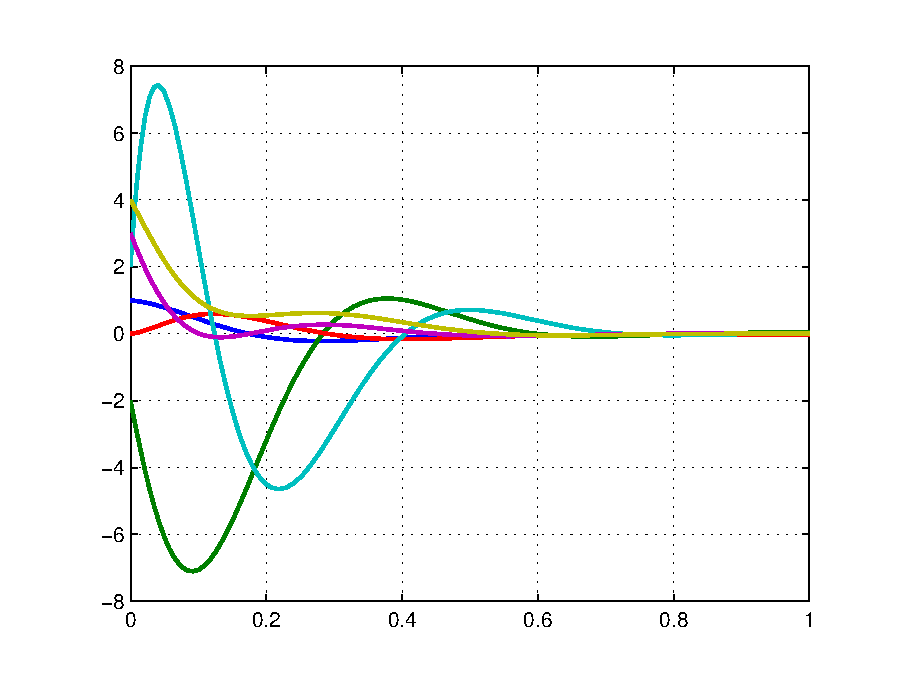
\includegraphics[width=0.6\textwidth]{Process}

   \vspace{-4mm}
  \caption{\small �������� ������� � ���������� $\widehat{u}=\widehat{K}_*\widehat{y}$ $(l=2, r=2)$.} \label{fig-2}
  \end{center}
\end{figure}

� ������� (a) ������� ����������� (\ref{s3-7}) ���������� � �������� ��������� ����������, �� ���������� �������� ��������� $J_1$ � $J_2$ �� ����� ������� ���������. �������������� ������� {\sc Matlab}, �������� ������� ��������� �������
$$
\widehat{P}=\left[\begin{array}{ccc}
    22,5659  &  0,1916  &  0,0992\\
    0,1916  & 21,2356 &   0,2037\\
    0,0992 &   0,2037  & 23,4494
    \end{array}
\right]>0,$$
$$\widehat{Q}=\left[\begin{array}{cccc}
     0,2397 &  -0,0005 &  -0,0009 &   0,0013\\
   -0,0005  &  0,2391  & -0,0007  &  0,0013\\
   -0,0009  & -0,0007  &  0,2256  &  0,0161\\
    0,0013  &  0,0013  &  0,0161  &  0,2215
    \end{array}
\right]>0,$$
$$ \widehat{X}= \left[\begin{array}{rrrrrr}
    4212,1  & -113,4 &  -4165,1 &  -191,1  &  66,7  &  19,2\\
   -113,4  &  21,8  &  124,4  &  1,1 &  -8,8 &  -10,2\\
   -4165,1  &  124,4  &  4250  &  193,5  & -59,1  & -5,6\\
   -191,1 &   1,1  &  193,5  &  19,2  &  5,2  &  5,4\\
    66,7  & -8,8  & -59,1  &  5,2  &  232,1  & -46,1\\
    19,2 &  -10,2  & -5,6  &  5,4  & -46,1  &  181,6
\end{array}
\right]>0,
$$
�� ������������� ������� ������� ������� ���������� ��� $\varepsilon_0=0$.
 ��� ��� ������� ������� ������� �� ������� ��������� � �������
 \begin{equation}\label{e1-4}
   \widehat{K}=\widehat{K}_*+\widetilde{K}, \quad \widetilde{K}^T\widehat{P}\widetilde{K}\le \widehat{Q},
 \end{equation}
 �� ���������� ����������� ������� ����������� ���������� ����������,
��� ������-������������ � ���� ��������� ����� �������� ������������ ������. ��� ����� $v(\widehat{x})=\widehat{x}^T\widehat{X}\widehat{x}$ � ������� �������� �������� ������� `����� -- ��������� ���������', � �������� �������� ����������� ����� �� �������� $v(\widehat{x}_0)=5753,6$.

� ������� (b) ������� ����������� (\ref{s3-7}) ���������� � ������ ��������� ����������, �� ���������� ��� �������� ��������� ��������� $k$, $d$ � $q$ �� ����� ������� ���������.
�������������� ������� {\sc Matlab}, �������� ������� ��������� �������
$$
\widehat{P}=\left[\begin{array}{ccc}
9,7612 &   0,1239  &  0,0518\\
    0,1239  &  9,7596 &   0,0086\\
    0,0518  &  0,0086  &  9,9692
    \end{array}
\right],$$
$$\widehat{Q}=\left[\begin{array}{cccc}
0,2216 &  -0,0012  & -0,0004 &   0,0012\\
   -0,0012 &   0,2197  & -0,0000 &   0,0013\\
   -0,0004 &  -0,0000 &   0,2076  &  0,0060\\
    0,0012  &  0,0013 &   0,0060  &  0,2067
 \end{array}
\right],$$
$${\widehat{X}\!\!=\!\!\left[\!\!\begin{array}{rrrrrr}
391,1327 & \!\!-11,8391& \!\!-368,5722 &  \!\!-8,0809 & \!\! -3,3290 &   1,0377\\
  -11,8391&    3,9551 &  22,9472  &  0,5287  &  0,3956 &   0,2964\\
 \!\!-368,5722 &  22,9472 & 492,5069  & 11,2335  &  5,8904  &  0,5692\\
   -8,0809  &  0,5287 &  11,2335  &  0,9488  &  0,5909  &  0,3985\\
   -3,3290 &   0,3956 &   5,8904   & 0,5909  & 14,5623  & \!\!-3,5012\\
    1,0377  &  0,2964  &  0,5692  &  0,3985  & \!\!-3,5012  & 10,1013\\
\end{array}
\!\!\right]\!,}
$$
�� ������������� ������� ������� ������� ���������� ��� $\varepsilon_0=0$.
 ��� ��� ������� ��������� $k$, $d$ �� $q$ �� ������� ���������
� ������� (\ref{e1-4}), �� ���������� ����������� ������� ����������� ���������� ����������,
��� ������-������������ � ���� ��������� ����� �������� ������������ ������. ��� ����� $v(\widehat{x})=\widehat{x}^T\widehat{X}\widehat{x}$ � ������� �������� �������� ������� `����� -- ��������� ���������', � �������� �������� ����������� ����� �� �������� $v(\widehat{x}_0)=767,7325$.

%%%%%%%%%%%%%%%%%%%%%%%%%%%%%%%%%%%%%%%%%%%%%%%%%%%%%%
%----------------------------------------------------------------

\medskip

����������, �� ������ (\ref{e1-2}) ���������� �������� ��������
$$y=Cx+Du=\left[\!\begin{array}{c}
                    \dot{\theta}_2+0,1\,\,\,u
                \end{array}
    \!\right],\> C=\left[\!\begin{array}{cccc}
                            0 & 0 & 0 & 1
                          \end{array}
    \!\right],\> D=\left[\!\begin{array}{c}
                            0,1
                        \end{array}
    \!\right].
$$
� ����� ������� �������� ���������� ��������� � ������ ���������� ���������� ������� ������� $r=n=4$, ����'������ ������� ����������� ������� $\widehat{X}=\widehat{X}^T>0$ � $\widehat{K}$ ��� $\alpha=-0,1$.
%$$ \widehat{X}= \left[\begin{array}{rrrrrrrr}
%5,4259 & -2,5720 & 5,5419 & -1,3028 & 0 & 0 & 0 & 0 \\
%-2,5720 & 15,9692 & -2,7705 & -0,7678 & 0 & 0 & 0 & 0\\
%5,5419 & -2,7705 & 5,8346 & -2,7266 & 0 & 0 & 0 & 0\\
%-1,3028 & -0,7678 & -2,7266 & 19,7167 & 0,5 & 0,5 & 0,5 & 0,5\\
%0 & 0 & 0 & 0,5 & 10 & 0 & 0 & 0\\
%0 & 0 & 0 & 0,5 & 0 & 10 & 0 & 0\\
%0 & 0 & 0 & 0,5 & 0 & 0 & 10 & 0\\
%0 & 0 & 0 & 0,5 & 0 & 0 & 0 & 10
%\end{array}
%\right]>0,
%$$
%$$
%\widehat{K}=\left[\begin{array}{ccccc}
%-4,2481 & 26,0307 & 26,4636 & 30,45 & 0,1392\\
%-26,0453 & -4,2481 & 1,5846 & -1,8407 & 0,1392\\
%-26,4782 & -1,5992 & -4,2481 & -4,1309 & 0,1392\\
%-30,4646 & 1,8261 & 4,1163 & -4,2481 & 0,1392\\
%-0,8042 & 0,8345 & 0,9231 & 0,8078 & -9.23
%                  \end{array}\right],
%$$
��� �����
$$
\widehat{K}_*\!=\!-\mathcal{\widehat{D}}(\widehat{K})\!=\!\left[\!\begin{array}{ccccc}
-4,1027 & \!25,8798 & \!26,2967 & 30,304 & 1,8078\\
-25,8999 & \!-4,3989 & 1,4177 & \!\!-1,9868 & 1,8078\\
-26,3328 & \!-1,7501 & -4,415 & \!\!-4,2769 & 1,8078\\
-30,3193 & 1,6753 & 3,9494 & \!\!-4,3941 & 1,8078\\
-10,4439 & 10,8384 & 11,9892 & 10,4918 & \!\!\!-119,8742
\end{array}\!\right]\!,
$$
$\widehat{K}_* \in {\mathcal K}_{\widehat{D}}$, $i(\widehat{H})=\{5,5,0\}$ � ��������� $\widehat{u}=\widehat{K}_*\widehat{y}$ ��������� ������������ ������� ������ ������� (\ref{e1-2-1}) (���. ���� \ref{lem:2}), ������ ���
$\sigma(\widehat{M}_*)=\{ -0,5489; -4,2406\pm 0,2145 i; -7,2319\pm 11,6669 i; -16,12;$ $ -4,2393\pm 48,262 i\}.
$
�������� ���� ������� �������� ������� (\ref{e1-2}) ����� � ��������� ����������� ����� ������������ ������. �� ���. \ref{fig-3} ��������� �������� ����'���� �������� �������� ������� (\ref{s2-6}) � ���������� ��������\\
$\widehat{x}_0=[0,5\>\>1\>\>1,5\>\>2\>\>-0,5\>\>-1\>\>-1,5\>\>-2]^T$.


�������� ��������� ���������� ���������� � ����������� �������� (a) � (b) ������������� ��������� ������� � ���� � ��������� ����������� (\ref{s3-1}), �� � � ������������ ������.

     \begin{figure}[ht]
  \begin{center}
  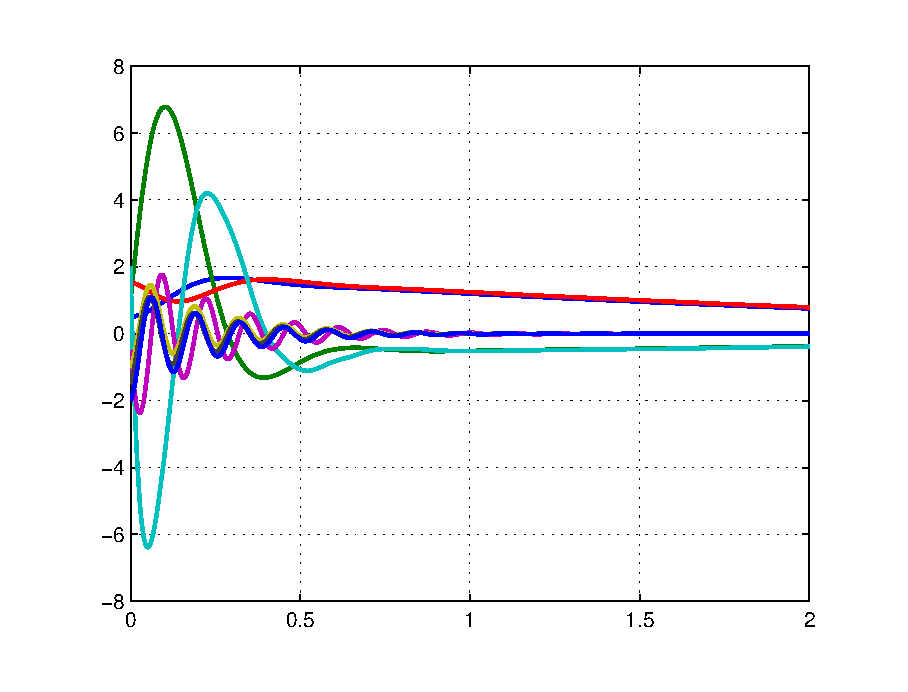
\includegraphics[width=0.6\textwidth]{Process_n}

   \vspace{-4mm}
  \caption{\small �������� ������� � ���������� $\widehat{u}=\widehat{K}_*\widehat{y}$ $(l=1, r=4)$.} \label{fig-3}
  \end{center}
\end{figure}

� ������� (a) ������� ��������� �������
$$
\widehat{P}=\left[\begin{array}{ccccc}
138,9143 & -0,0906 & -0,8891 & 0,8471 & 0,0699\\
-0,0906 & 130,4898 & 3,4543 & 4,2867 & 0,1607\\
-0,8891 & 3,4543 & 130,5692 & 4,3979 & 0,1386\\
0,8471 & 4,2867 & 4,3979 & 131,5409 & 0,3647\\
0,0699 & 0,1607 & 0,1386 & 0,3647 & 123,2942
    \end{array}
\right],$$
$$\widehat{Q}=\left[\begin{array}{ccccc}
0,024 & 0 & 0 & 0 & 0\\
0 & 0,024 & 0 & 0 & 0\\
0 & 0 & 0,024 & 0 & 0\\
0 & 0 & 0 & 0,024 & 0\\
0 & 0 & 0 & 0 & 0,024
    \end{array}
\right],$$
$$ \widehat{X}\!= \!\left[\begin{array}{rrrrrrrr}
1834,2 & \!\!-39,4 & \!\!-1795,5 & \!\!-62 & \!\!-11,9 & -7,2 & -7,4 & -4\\
-39,4 & 9,4 & 41,5 & -1 & 0,7 & 0,4 & 0,5 & -0,6\\
\!\!\!-1795,5 & 41,5 & \!\!1766,9 & 61 & 12,3 & 6,8 & 6,8 & 5,2\\
-62 & -1 & 61 & 5,2 & \!\!\!-1,7 & 1,5 & 1,8 & 1,2\\
-11,9 & 0,7 & 12,3 & \!\!-1,7 & 573,2 & -2,2 & -2,6 & 3,6\\
-7,2 & 0,4 & 6,8 & 1,5 & -2,2 & 576,6 & \!\!-16,4 & 9,8\\
-7,4 & 0,5 & 6,8 & 1,8 & -2,6 & \!\!-16,4 & \!\!564,3 & 20,1\\
-4 & -0,6 & 5,2 & 1,2 & 3,6 & 9,8 & 20,1 & \!\!545,8
\end{array}
\right]\!,
$$
������������� ������� ������� ���������� (\ref{s3-7}) ��� $\varepsilon_0=0$.
 ��� ��� ������� ������� ������� $J_1$ � $J_2$ �� ������� ��������� � ������� $\widehat{K}$
 �� ���������� ����������� ������� ����������� (\ref{e1-4}) ���������� ����������,
��� ������-������������ � ���� ��������� ����� �������� ������������ ������. ��� ����� $v(\widehat{x})=\widehat{x}^T\widehat{X}\widehat{x}$ � ������� �������� �������� �������, � �������� �������� ����������� ����� �� �������� $v(\widehat{x}_0)=6286,5$.

� ������� (b) ������� ������� ��������� �������
$$
\widehat{P}=\left[\begin{array}{ccccc}
139,6246 & -0,0579 & -0,6031 & 0,5661 & 0,1813\\
-0,0579 & 133,8658 & 2,4128 & 2,8851 & 0,1823\\
-0,6031 & 2,4128 & 133,9549 & 2,9319 & 0,1724\\
0,5661 & 2,8851 & 2,9319 & 134,6888 & 0,25\\
0,1813 & 0,1823 & 0,1724 & 0,25 & 125,7135
    \end{array}
\right],$$
$$\widehat{Q}=\left[\begin{array}{ccccc}
0,022 & 0 & 0 & 0 & 0\\
0 & 0,022 & 0 & 0 & 0\\
0 & 0 & 0,022 & 0 & 0\\
0 & 0 & 0 & 0,022 & 0\\
0 & 0 & 0 & 0 & 0,022
 \end{array}
\right],$$
$$ \widehat{X}= \left[\begin{array}{rrrrr}
334,6812 & -10,8539 & -315,8285 & -6,7508 & -12,6088     \\
-10,8539 & 3,539 & 20,4582 & 0,5119 & 0,3484            \\
-315,8285 & 20,4582 & 418,8241 & 9,4635 & 11,7803        \\
-6,7508 & 0,5119 & 9,4635 & 0,777 & -1,8269             \\
-12,6088 & 0,3484 & 11,7803 & -1,8269 & 551,6656        \\
-5,9544 & 0,1809 & 5,3233 & 1,3361 & -2.081             \\
-5,7255 & 0,3652 & 4,9185 & 1,4952 & -6,7576            \\
-4,8031 & -0,768 & 5,27 & 1,3844 & 7,214
\end{array}
\right.
$$
$$ \left. \begin{array}{rrr}
       -5,9544 & -5,7255 & -4,8031\\
               0,1809 & 0,3652 & -0,768\\
        5,3233 & 4,9185 & 5,27\\
             1,3361 & 1,4952 & 1,3844\\
         -2.081 & -6,7576 & 7,214\\
              508.8325 & 6,1446 & 29,8012\\
             6,1446 & 499,3528 & 38,8969\\
                29,8012 & 38,8969 & 490,055
\end{array}
\right],
$$
������������� ������� ������� ���������� (\ref{s3-7}) ��� $\varepsilon_0=0$.
 ��� ��� ������� ��������� $k$, $d$ �� $q$ �� ������� ���������
� ������� $\widehat{K}$, �� ���������� ����������� ������� ����������� (\ref{e1-4}) ���������� ����������,
��� ������-������������ � ���� ��������� ����� �������� ������������ ������. ��� ����� $v(\widehat{x})=\widehat{x}^T\widehat{X}\widehat{x}$ � ������� �������� �������� �������, � �������� �������� ����������� ����� �� �������� $v(\widehat{x}_0)=5409,3$.

%--------------------------------------------------------------
%�������������� ����� �������� ���� \ref{lem:3} ��� ������ ���������, �� ������� ������� (\ref{e1-2}), ����������� ���� � ������ ��� (\ref{s1-2}) ��� $r=n=4$ ��� ���� � ������ ������, �� � � ������������ ������.
%
%����'������ �� ��� (\ref{s1-19}) ��������� ������� $X$ � $Y$:
%$$X=\left[\begin{array}{cccc}
%0,417 & -0,1088 & 0,4195 & -0,0979\\
%-0,1088 & 1,8136 & -0,1197 & 0,804\\
%0,4195 & -0,1197 & 0,4324 & -0,1316\\
%0,0979 & 0,804 & -0,1316 & 4,2435
% \end{array}
%\right]>0,$$
%$$Y=\left[\begin{array}{cccc}
%2,5408 & -0,2689 & -0,117 & -0,0863\\
%-0,2689 & 0,5338 & 0,4437 & 0,1601\\
%-0,117 & 0,4437 & 1,3287 & 0.1347\\
%-0,0863 & 0,1601 & 0,1347 & 0,0515
%\end{array}
%\right]>0.$$
%
%�������� � ������������� (\ref{s1-18}) $K=0$, ��������� ������� $U$ � $F$, � � (\ref{s1-15}) --- ������� $Z$ �� $V$. ����, ��������, ��
%$$
%\widehat{K}=\left[\begin{array}{ccccc}
%-0,1654 & 0,974 & 0,1721 & -0,643 & 0,7048\\
%-84,8469 & 3,1634 & 79,0308 & 78,3444 & -85,8747\\
%0,13 & 0,0204 & -0,1353 & 1,5056 & -0,5541\\
%273,3298 & -9,4187 & -270,9001 & -266,9281 & 289,0154\\
%2,3468 & 0,3684 & -2,4418 & -0,8769 & 0
%                  \end{array}\right].
%$$
%��� �����
%$$
%\widehat{K}_*=-\mathcal{\widehat{D}}(\widehat{K})=\left[\!\begin{array}{ccccc}
%0 & 1 & 0 & -0,7048 & 0,7048\\
%-105 & 0 & 100 & 85,8747 & -85,8747\\
%0 & 0 & 0 & 1,5541 & -0,5541\\
%341,156 & 1,2279 & -341,4728 & -292,2717 & 289,0154\\
%2,3468 & 0,3684 & -2,4418 & -0,8769 & 0
%\end{array} \!\right]\in {\mathcal K}_{\widehat{D}},
%$$
%� ��������� $\widehat{u}=\widehat{K}_*\widehat{y}$ ��������� ������������ ������� ��������� ����� ������� \ref{s1-2}. �� ���. \ref{fig-4} ��������� �������� ����'���� �������� �������� ������� (\ref{s2-2}) � ���������� �������� $\widehat{x}_0~=~[0,5\>\>1\>\>1,5\>\>2\>\>-~0,5\>\>-~1\>\>-1,5\>\>-2]^T$.
%
%��� ���������� ������� \ref{the:2} ������ ������ ������� $\widehat{S}$, $\widehat{R}$ � $\widehat{N}$ ����������� (\ref{s3-1}) � ������ (\ref{s3-2-1}) ��� ��� �� ����� ���������, �� � � ������������ ������. ����� ���������� ��� ������� ���� ���������:
%
%  (a) $J_1$ � $J_2$ --- ����������� ������� �������, �� ��������� �������� �� ���������� $0,99 \leq J_1 \leq 1,03$ � $0,2\leq J_2\leq 0,5$;
%
% (b) $k$, $d$ � $q$ --- ����������� ���������, �� ��������� �������� �� ���������� $99\leq k \leq 101$,\,\, $0,05\leq d\leq 0,2$ � $4\leq q\leq 6$.
%
%     \begin{figure}[h!]
%  \begin{center}
%  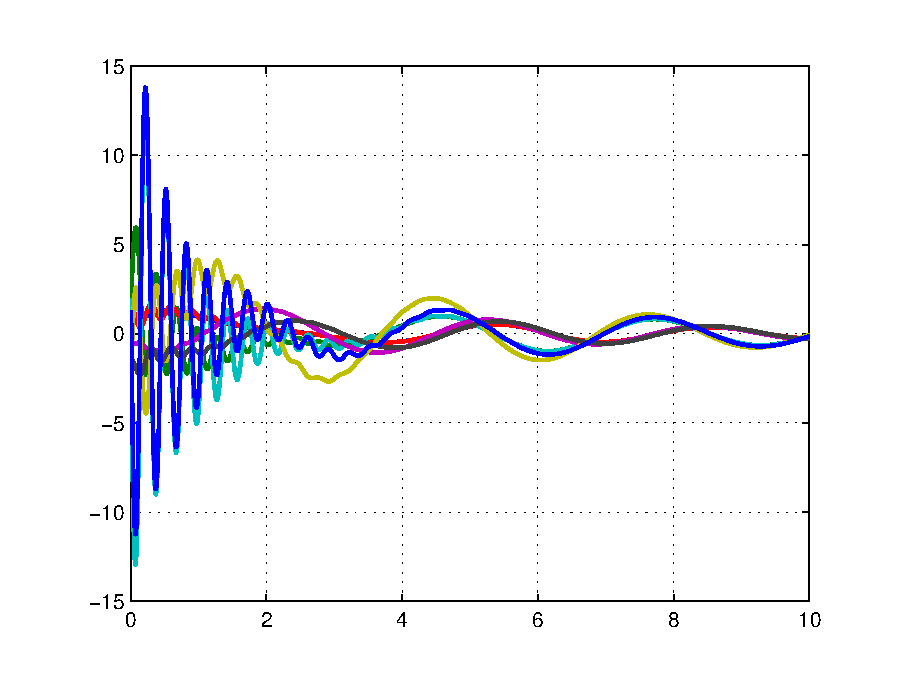
\includegraphics[width=0.6\textwidth]{Process_s}
%
%   \vspace{-4mm}
%  \caption{\small �������� ������� � ���������� $\widehat{u}=\widehat{K}_*\widehat{y}$.} \label{fig-4}
%  \end{center}
%\end{figure}
%
%� ������� (a) ������� ����������� (\ref{s3-7}) ���������� � �������� ��������� ����������, �� ���������� �������� ��������� $J_1$ � $J_2$ �� ����� ������� ���������. �������������� ������� {\sc Matlab}, �������� ������� ��������� �������
%$$
%\widehat{P}=\left[\begin{array}{ccccc}
%957,7013 & -8,3454 & 6,6341 & -3,2026 & 0,4243\\
%-8,3454 & 893,8336 & 22,2302 & 17,9093 & -2,0183\\
%6,6341 & 22,2302 & 919,3079 & 7,4926 & -0,7439\\
%-3,2026 & 17,9093 & 7,4926 & 840,1426 & 1,7368\\
%0,4243 & -2,0183 & -0,7439 & 1,7368 & 993,5286
%\end{array}
%\right]>0,$$
%$$\widehat{Q}=\left[\begin{array}{ccccc}
%0,0015 & 0 & 0 & 0 & 0\\
%0 & 0,0015 & 0 & 0 & 0\\
%0 & 0 & 0,0015 & 0 & 0\\
%0 & 0 & 0 & 0,0015 & 0\\
%0 & 0 & 0 & 0 & 0,0015
%    \end{array}
%\right]>0,$$
%$$ \widehat{X}= \left[\begin{array}{rrrrrrrr}
%50539 & -190 & -49189 & -396 & -579 & 254 & 213 & 146\\
%-190 & 350 & 365 & -47 & 115 & -157 & -306 & -44\\
%-49189 & 365 & 49423 & 452 & 221 & -376 & -923 & -189\\
%-396 & -47 & 452 & 549 & 510 & -55 & -572 & -415\\
%-579 & 115 & 221 & 510 & 1524 & -169 & -1231 & -510\\
%254 & -157 & -376 & -55 & -169 & 160 & 326 & 54\\
%213 & -306 & -923 & -572 & -1231 & 326 & 2016 & 564\\
%146 & -44 & -189 & -415 & -510 & 54 & 564 & 404
%\end{array}
%\right]>0,
%$$
%�� ������������� ������� ������� ������� ���������� ��� $\varepsilon_0=0$.
% ��� ��� ������� ������� ������� �� ������� ��������� � �������
% \begin{equation}\label{e1-4}
%   \widehat{K}=\widehat{K}_*+\widetilde{K}, \quad \widetilde{K}^T\widehat{P}\widetilde{K}\le \widehat{Q},
% \end{equation}
% �� ���������� ����������� ������� ����������� ���������� ����������,
%��� ������-������������ � ���� ��������� ����� �������� ������������ ������. ��� ����� $v(\widehat{x})=\widehat{x}^T\widehat{X}\widehat{x}$ � ������� �������� �������� ������� `����� -- ��������� ���������', � �������� �������� ����������� ����� �� �������� $v(\widehat{x}_0)=76221$.
%
%� ������� (b) ������� ����������� (\ref{s3-7}) ���������� � ������ ��������� ����������, �� ���������� ��� �������� ��������� ��������� $k$, $d$ � $q$ �� ����� ������� ���������.
%�������������� ������� {\sc Matlab}, �������� ������� ��������� �������
%$$
%\widehat{P}=\left[\begin{array}{ccccc}
%1190,4 & -7,8 & 15,5 & -2,9 & 1,2\\
%-7,8 & 1163,8 & 23,7 & 27,9 & -1,5\\
%15,5 & 23,7 & 1143,8 & 7,4 & -0,6\\
%-2,9 & 27,9 & 7,4 & 178 & 0,9\\
%1,2 & -1,5 & -0,6 & 0,9 & 1191,9
%\end{array}
%\right]>0,$$
%$$\widehat{Q}=\left[\begin{array}{ccccc}
%0,0011 & 0 & 0 & 0 & 0\\
%0 & 0,0011 & 0 & 0 & 0\\
%0 & 0 & 0,0011 & 0 & 0\\
%0 & 0 & 0 & 0,0011 & 0\\
%0 & 0 & 0 & 0 & 0,0011
% \end{array}
%\right]>0,$$
%$$ \widehat{X}= \left[\begin{array}{rrrrrrrr}
%49430 & -385 & -48839 & -503 & -589 & 375 & 729 & 272\\
%-385 & 245 & 522 & -76 & 141 & -105 & -293 & -24\\
%-48839 & 522 & 49117 & 545 & 611 & -478 & -1408 & -308\\
%-503 & -76 & 545 & 607 & 609 & -38 & -658 & -483\\
%-589 & 141 & 611 & 609 & 1538 & -194 & -1432 & -604\\
%375 & -105 & -478 & -38 & -194 & 142 & 335 & 46\\
%729 & -293 & -1408 & -658 & -1432 & 335 & 2225 & 651\\
%272 & -24 & -308 & -483 & -604 & 46 & 651 & 475
%\end{array}
%\right]>0,
%$$
%�� ������������� ������� ������� ������� ���������� ��� $\varepsilon_0=0$.
% ��� ��� ������� ��������� $k$, $d$ �� $q$ �� ������� ���������
%� ������� (\ref{e1-4}), �� ���������� ����������� ������� ����������� ���������� ����������,
%��� ������-������������ � ���� ��������� ����� �������� ������������ ������. ��� ����� $v(\widehat{x})=\widehat{x}^T\widehat{X}\widehat{x}$ � ������� �������� �������� ������� `����� -- ��������� ���������', � �������� �������� ����������� ����� �� �������� $v(\widehat{x}_0)=47291$.

%---------------------------------------------------------------
%%%%%%%%%%%%%%%%%%%%%%%%%%%%%%%%%%%%%%%%%%%%%%%%%%%%%%

���������, �� ��� ������ ��������� ������������ ��� � �������� $K_*$ ������� ��� $\widehat{K}_*$ ����� �������� � ������
 $$\widehat{K}_*=\left[\!\begin{array}{cc}
              Z_* & 0_{r\times l} \\
              0_{m\times r} & K_*
            \end{array} \!\right],$$
�� $Z_*\in {\mathbb R}^{r\times r}$ --- ������� ������� � �������� � ��� ����������� $\{\lambda\in {\mathbb C}^1:\,{\rm Re} \lambda <0\}$.

\section{��������}

� ����� �������� ��� ������ ������ �������� ������� ������ �������� � ���������� ��������� ������ ��������� � ��������� ��������� ��'����� �� ������. ��� ����� �������� ������������ ��������� ����������� ������ �������� ������� ��������, �������, ��������� ���������� ��� ������� ��������, � ������ �������� ������� ����������� ���������� ���������� �������� ����������� �������. ������ ���������� � ���������� � ��������� ����������� ��������� ������� ������� �� ���������� ����� � ��������� ��������� ��'����� � ��������� ������ ������.

��������� ��������� �������������� ������ �������� �� ����'������ ��������������� ��� ����������� ���. ��� ����������� ����'���� ����������� ��� ���� ���� ����������� ��������� ��������� ��������� � ������ {\sc Matlab}. ³������ ���������� ����������� ��� �� ������ � ��������� �������� ������� ������� ���������� ���������� ��'����, ������ ����������� ������� ��������, � ����� ������ ������������� ����������� ����� ��� �������� ������� ��������� � ������������� ���������� �������������.

{\small

\renewcommand\refname{}

\begin{thebibliography}{99}

\bibitem{Polyak-Scherbakov} \emph{����� �.�., �������� �.�.}  ��������� ������������ � ����������. --- �.: �����, 2002. --- 303 �.

\bibitem{Zhou-Doyle-Glover} \emph{Zhou K., Doyle J.C., Glover K.}  Robust and optimal
control. --- Englewood: Prentice-Hall, Inc., 1996. --- 586 p.

\bibitem{Kuncevich} \emph{�������� �.�.} ���������� � �������� ����������������: ��������������� ���������� � ������� ���������� � �������������. --- ����: ����. �����, 2006. --- 264 �.

\bibitem{Polyak-Scherbakov-1} \emph{����� �.�., �������� �.�.}  ������� ������ �������� ������ ����������. ��������� ������� � ������� // ���������� � ������������. --- 2005. --- � 5. --- �. 7--46.

\bibitem{Aliev-Larin} \emph{����� �.�., ����� �.�.}  ������ ������������ ������� � �������� ������ �� �������� ���������� (�����) // ���������� ��������. --- 2011. --- �. 47, � 3. --- �. 3--49.

\bibitem{Mazko-2008} \emph{Mazko A.G.}  Matrix Equations, Spectral Problems and Stability of Dynamic Systems.
 An international book series ``Stability, Oscillations and Optimization of Systems''. A.A. Martynyuk, P. Borne and C. Cruz-Hernandez, eds. V. 2. --- Cambridge: Cambridge Scientific Publishers Ltd, 2008. --- XX+270 p.

 \bibitem{Mazko-2011} \emph{Mazko A.G.} Cone inequalities and stability of dynamical systems //  Nonlinear Dynamics and Systems Theory. --- 2011. --- V. 11, �~3. --- P. 303--318.

\bibitem{Balandin-Kogan} \emph{�������� �.�., ����� �.�.}  ������ ������� ���������� �� ������ �������� ��������� ����������. --- �.: ���������, 2007. --- 280 c.

\bibitem{Maz-Shram-2011} \emph{����� �.�., ���� �.�.} ������������ � ������������ ��������� �������������� ���������������� ������ // ���������� ���������. --- 2011. --- �. 14, � 2. --- C.~227--237.

\bibitem{Mazko-2011-IM}  \emph{����� �.�.} ��������� ������������ � ������ �������� ��������� ���������� ������ ���������� // �������� ������� �� ������� ������������� ������: ������ ����� ��-�� ����������  ��� ������. --- 2011.~--- �. 8, � 2. --- �. 174--186.

\bibitem{Maz-Bog-2012} \emph{����� �.�., ���������� �. �. }
 �������� ������� � ���������� ��������� ������ ��������� // ��������� �������� �� �� ������������: ������ ����� I�-�� ���������� ��� ������. --- 2012. --- �. 9, � 1. --- �. 200--218.

 \bibitem{Gu-Petkov-Konstantinov} \emph{Gu D.-W., Petkov P. Hr.  and Konstantinov M. M.}
\emph{Robust Control Design with MATLAB}. --- Springer-Verlag London Limited, 2005. --- 389 p.

 \bibitem{El-Ghaoui-Gahinet-1993} \emph{El-Ghaoui L., Gahinet P.} Rank minimization under LMI constraints: a framework for output feedback problems. In: Proc. Eur. Control Conf. Groningen, The Netherlands, 1993. --- P. 1176--1179.

\bibitem{Petersen} \emph{Petersen I.} A stabilization algorithm for a class of uncertain linear systems // Systems Control Lett. --- 1987. --- V. 8, � 4. --- P. 351--357.

\bibitem{Ghorbel}\emph{Ghorbel F., Hung J.Y., Spong M.W.} Adaptive control of flexible-joint manipulators // IEEE Control Systems Mag.--� 1989.--� � 9.--� P. 9�13.

\end{thebibliography}
}
%\label{Mazko-Kupriyanchyk:LastPage}

%\newpage
\end{document}
	%\input{./Mazko-Bogdanovych/Mazko-Bogdanovych}
	
	\def\enddocument{\oldenddocument}
\end{document}
